\documentclass[fontsize=12pt, DIV=15, parskip=half-]{scrartcl}

\usepackage[utf8]{inputenc}
\usepackage[english, german]{babel}
\usepackage[T1]{fontenc}
\usepackage{lmodern}
\usepackage[lf]{libertine}
\usepackage{pgfpages}
\usepackage{tikz}
\usepackage{textcomp}
\usepackage{microtype}
\usepackage{array}
\usepackage[inline]{enumitem}
\usepackage[intlimits]{amsmath}
\usepackage{amssymb}
\usepackage{amsfonts}
\usepackage[amsmath, thmmarks]{ntheorem}
\usepackage[italic, defaultmathsizes, basic]{mathastext}
\usepackage{mathtools}
\usepackage{stmaryrd}
\usepackage{booktabs}
\usepackage{nicefrac}
\usepackage{ifthen}
\usepackage{suffix}
\usepackage{cancel}
\usepackage{setspace}
\usepackage{stmaryrd}
\usepackage{hyperref}
\usepackage{nameref}

\linespread{1.05}

\theoremstyle{break}
\theoremheaderfont{\sffamily\bfseries}
\theorembodyfont{\upshape}
\newtheorem{aufgabe}{Aufgabe}
\newtheorem{loesung}{Lösung zu Aufgabe}
\newtheorem{ergaufgabe}[aufgabe]{$^*$Aufgabe}
\newtheorem{ergloesung}[loesung]{Lösung zu Aufgabe}

\newcommand{\defin}[1]{\textbf{\textit{\color{blue}#1}}}
\newcommand{\anm}[1]{~~\hfill(#1)}
\newcommand{\defanm}[1]{~~\hfill\defin{(#1)}}
\newcommand{\N}{\mathbb{N}}
\newcommand{\Z}{\mathbb{Z}}
\newcommand{\Q}{\mathbb{Q}}
\newcommand{\R}{\mathbb{R}}
\newcommand{\C}{\mathbb{C}}
%\newcommand{\cal}[1]{\mathcal{#1}}
\newcommand{\tmenge}[2]{\smash{\{#1\mathbin|#2\}}}
\newcommand{\menge}[2]{\left\{#1\:\middle|\:#2\right\}}
\newcommand{\rk}[1]{\left(#1\right)}
\newcommand{\ro}[1]{\left[#1\right)}
\newcommand{\lo}[1]{\left(#1\right]}
\newcommand{\ab}[1]{\left[#1\right]}
\newcommand{\st}[1]{\stackrel{\text{#1}}}
\newcommand{\stm}[1]{\stackrel{#1}}
\newcommand{\imp}{\Rightarrow}
\newcommand{\timp}[1]{\overset{\text{#1}}{\imp}}
\newcommand{\kimp}[1]{\overset{\mathclap{\text{#1}}}{\imp}}
\newcommand{\aeq}{\Leftrightarrow}
\newcommand{\ait}{\quad\aeq\quad}
\newcommand{\stait}[1]{\quad\stackrel{#1}\aeq\quad}
\newcommand{\ohne}[1]{\setminus \{#1\}}
\newcommand{\tim}[1]{\text{\quad #1 \quad}}
\newcommand{\taeq}[1]{\overset{\text{#1}}{\aeq}}
\newcommand{\kaeq}[1]{\overset{\mathclap{\text{#1}}}{\aeq}}
\newcommand{\tg}[1]{\overset{\text{#1}}{=}}
\newcommand{\kg}[1]{\overset{\mathclap{\text{#1}}}{=}}
\newcommand{\eps}{\varepsilon}
\renewcommand{\phi}{\varphi}
\renewcommand{\rho}{\varrho}
\newcommand{\CCC}{\operatorname{C}}
\newcommand{\DDD}{\operatorname{D}}
\newcommand{\MMM}{\operatorname{M}}
\newcommand{\Pot}{\mathfrak{P}}
\newcommand{\id}{\mathrm{id}}
\renewcommand{\leq}{\leqslant}
\renewcommand{\geq}{\geqslant}
\newcommand{\eee}{\mathrm{e}}
\newcommand{\iii}{\mathrm{i}}
\newcommand{\modu}{~\mathrm{modulo}}
\newcommand{\dd}[1]{\:\mathrm{d}#1}
\newcommand{\dt}{\dd{t}}
\newcommand{\dx}{\dd{x}}
\newcommand{\dxyz}{\dd{(x, y, z)}}
\renewcommand{\Re}{\operatorname{Re}}
\renewcommand{\Im}{\operatorname{Im}}
\newcommand{\Grad}{\operatorname{Grad}}
\newcommand{\Kern}{\operatorname{Kern}}
\newcommand{\Bild}{\operatorname{Bild}}
\newcommand{\Hess}{\operatorname{Hess}}
\newcommand{\tbetr}[1]{\mathopen|\smash{#1}\mathclose|}
\newcommand{\betr}[1]{\left|#1\right|}
\newcommand{\mmn}[2]{\begin{pmatrix} #1 \\ #2 \end{pmatrix}}
\newcommand{\tmmn}[2]{\smash{(\begin{smallmatrix} #1 \\ #2 \end{smallmatrix})}}
\newcommand{\mmmn}[3]{\begin{pmatrix} #1 \\ #2 \\ #3 \end{pmatrix}}
\newcommand{\mmnn}[4]{\begin{pmatrix} #1 & #2 \\ #3 & #4 \end{pmatrix}}
\newcommand{\mnnnn}[4]{\begin{pmatrix} #1 & #2 & #3 & #4 \end{pmatrix}}
\newcommand{\mmmmn}[4]{\begin{pmatrix} #1 \\ #2 \\ #3 \\ #4 \end{pmatrix}}
\newcommand{\mmmnnn}[9]{\begin{pmatrix} #1 & #2 & #3\\ #4 & #5 & #6\\ #7 & #8 & #9 \end{pmatrix}}
\newcommand{\mmmnn}[6]{\begin{pmatrix} #1 & #2 \\ #3 & #4\\ #5 & #6 \end{pmatrix}}
\newcommand{\mmnnn}[6]{\begin{pmatrix} #1 & #2 & #3\\ #4 & #5 & #6 \end{pmatrix}}

\newenvironment{mathex}[1][LLLLLLLLLLLL]{
  \[%
  \newcolumntype{L}{>{\displaystyle\setlength{\arraycolsep}{4pt}}l}%
  \newcolumntype{C}{>{\displaystyle\setlength{\arraycolsep}{4pt}}c}%
  \newcolumntype{R}{>{\displaystyle\setlength{\arraycolsep}{4pt}}r}%
  \setlength{\arraycolsep}{1.5pt}%
  \begin{array}{>{\vspace*{1.3ex}}#1}%
}{
  \end{array}%
  \vspace*{-1.3ex}%
  \]%
  \ignorespacesafterend%
}

\newcommand{\sternitem}{\refstepcounter{enumi}\item[($^*$\alph{enumi})]}

\newcounter{paeckchenteil}
\newcounter{paeckcheninzeile}
\newenvironment{paeckchen}[1][3]{
\setcounter{paeckchenteil}{0}
\setcounter{paeckcheninzeile}{0}
\renewcommand{\item}{%
\ifthenelse{\value{paeckchenteil}=0}{}{&}%
\ifthenelse{\value{paeckchenteil}>0 \and \value{paeckcheninzeile}=0}{\\}{}%
\refstepcounter{paeckchenteil}%
\stepcounter{paeckcheninzeile}%
\ifthenelse{\value{paeckcheninzeile}=#1}{\setcounter{paeckcheninzeile}{0}}{}%
\text{(\alph{paeckchenteil})}%
&
}%
\WithSuffix\newcommand\item*{%
\ifthenelse{\value{paeckchenteil}=0}{}{&}%
\ifthenelse{\value{paeckchenteil}>0 \and \value{paeckcheninzeile}=0}{\\}{}%
\refstepcounter{paeckchenteil}%
\stepcounter{paeckcheninzeile}%
\ifthenelse{\value{paeckcheninzeile}=#1}{\setcounter{paeckcheninzeile}{0}}{}%
\text{($^*$\alph{paeckchenteil})}%
&
}%
\renewcommand{\sternitem}{\item*}
\begin{mathex}[R>{\;\;}L>{\qquad}R>{\;\;}L>{\qquad}R>{\;\;}L>{\qquad}R>{\;\;}L>{\qquad}R>{\;\;}L>{\qquad}R>{\;\;}L>{\qquad}R>{\;\;}L]
}{
\end{mathex}
}

%\pagestyle{empty}
\begin{document}
\begin{center}
\Large\bfseries\sffamily JavaCrypTool (\url{www.cryptool.org})

Online help for the usage of the grille analysis  \\[0.1\baselineskip]
\normalsize\normalfont 
\end{center}
\vspace*{0.5\baselineskip}

\selectlanguage{english}
\tableofcontents
\newpage

\selectlanguage{german}
The main function of this plug-in is the analysis of a ciphertext that has been encrypted using the grille cipher. The content of the template is used as key. Somewhat unusual here is the characterization of the key length as the side length of the square field (template).

In addition to the analysis function, the functions \hyperlink{verschl} {Encryption} and \hyperlink{entschl}{Decryption} are also available in this plug-in.


\section{Analysis}
In the initial setting of the plug-in (default setting), the radio button is set on the analysis function. It is selected in the first aggregation \glqq Method\grqq. The method can be changed to either encryption or decryption.

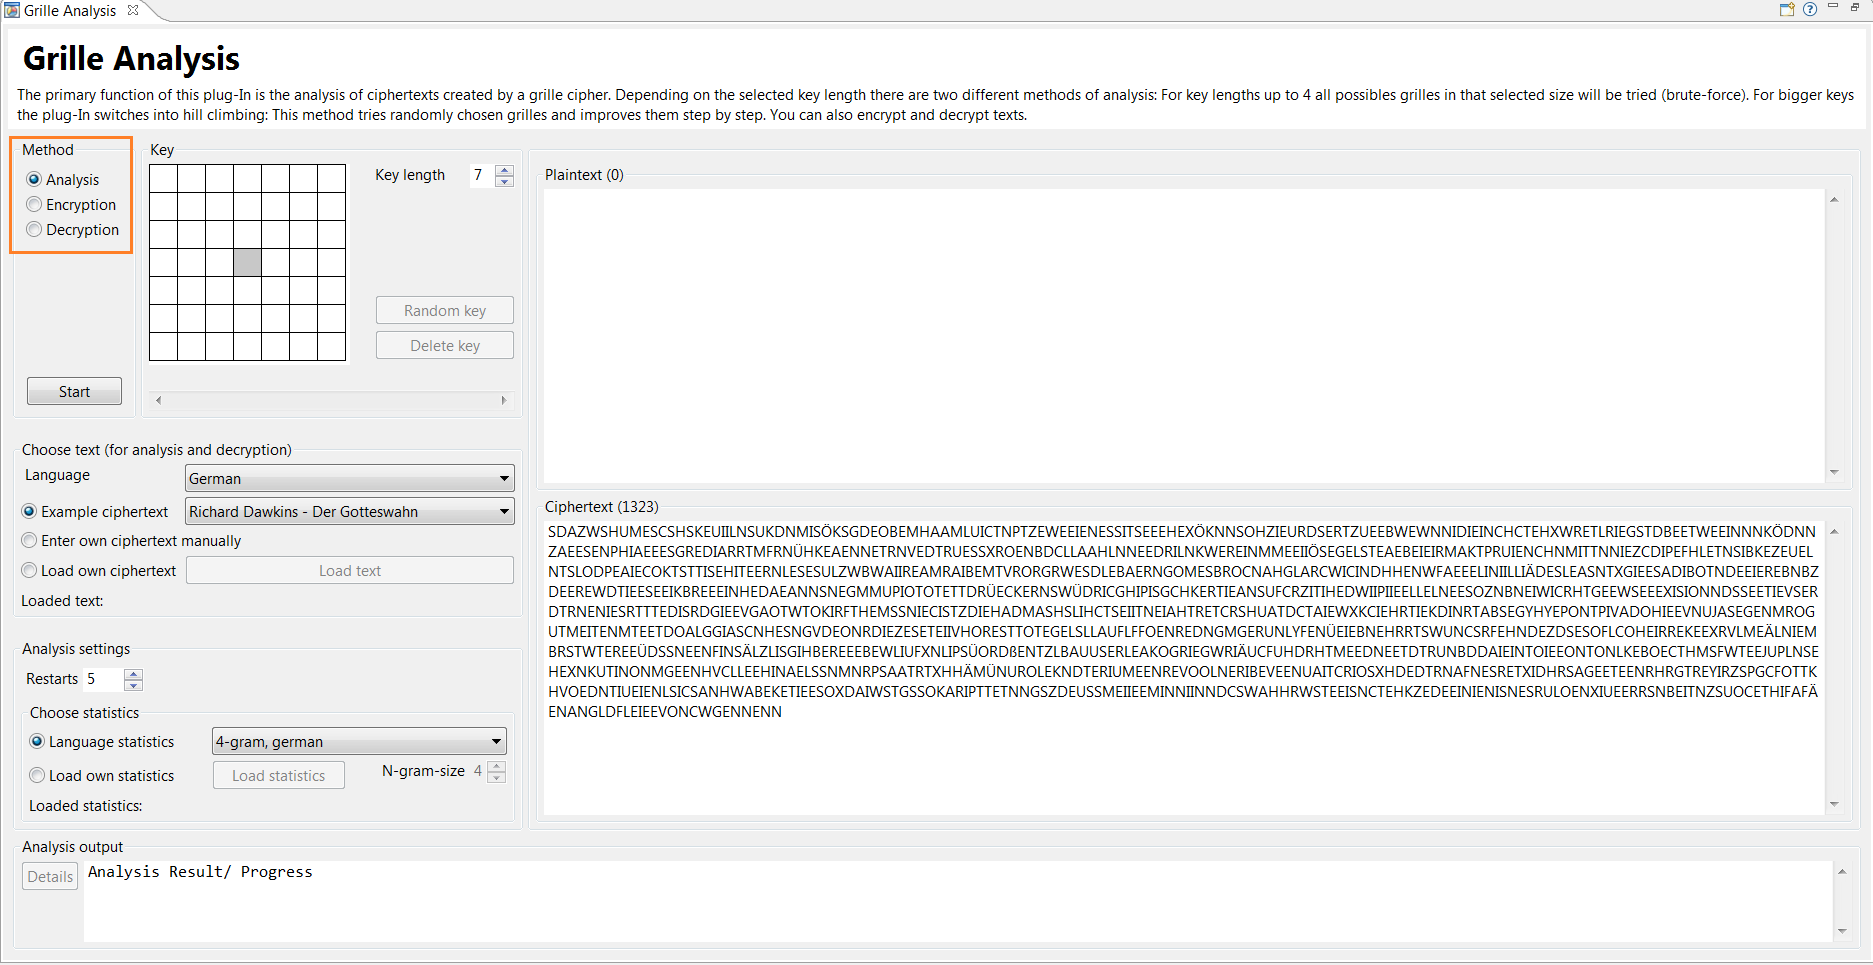
\includegraphics[scale=0.45]{enFleissnerMethods.png}
%\newpage

Every relevant parameter for the analysis as well as the ciphertext has a default setting, so as to start an analysis immediately by pressing the \glqq Start\grqq{} button below the method selection.

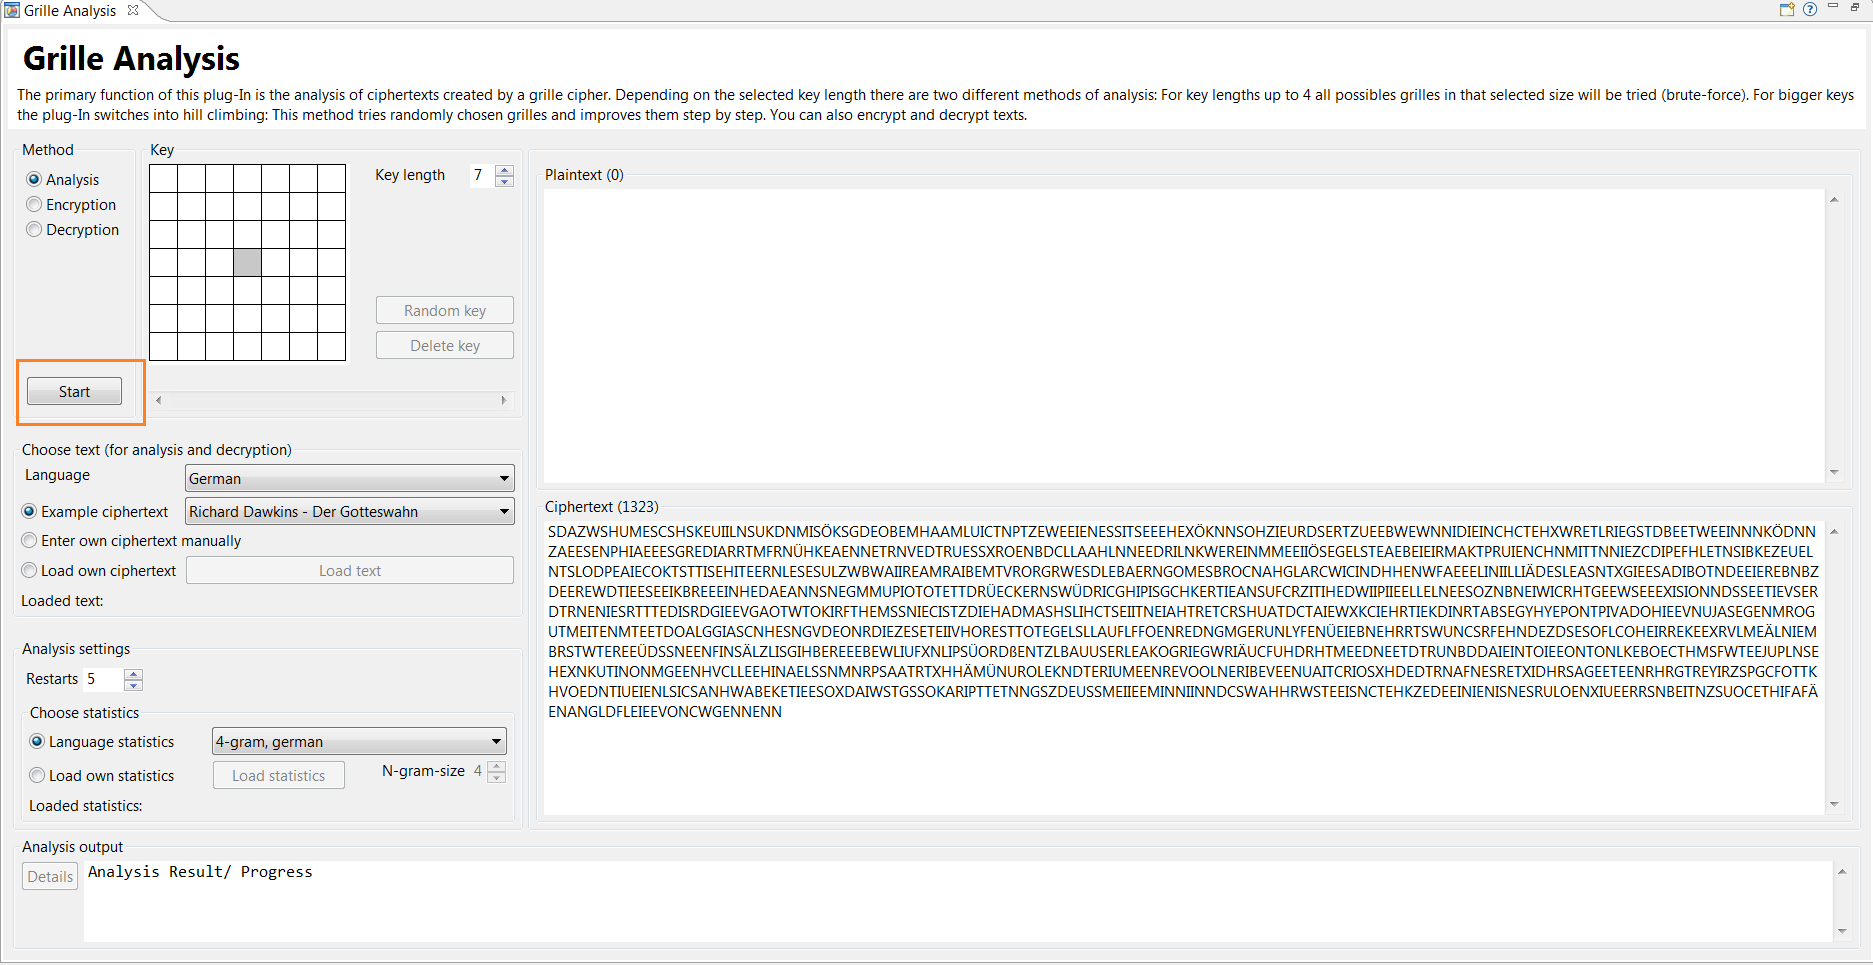
\includegraphics[scale=0.45]{enFleissnerStart.png}
%\newpage

\subsection{Key length}
Since the key used for encrypting the text is secret and is supposed to be found by the analysis, the key field itself is disabled for this method. 
However, the key length is important for a successful analysis and is made available next to the key field. This length should match that of the key used for this ciphertext.

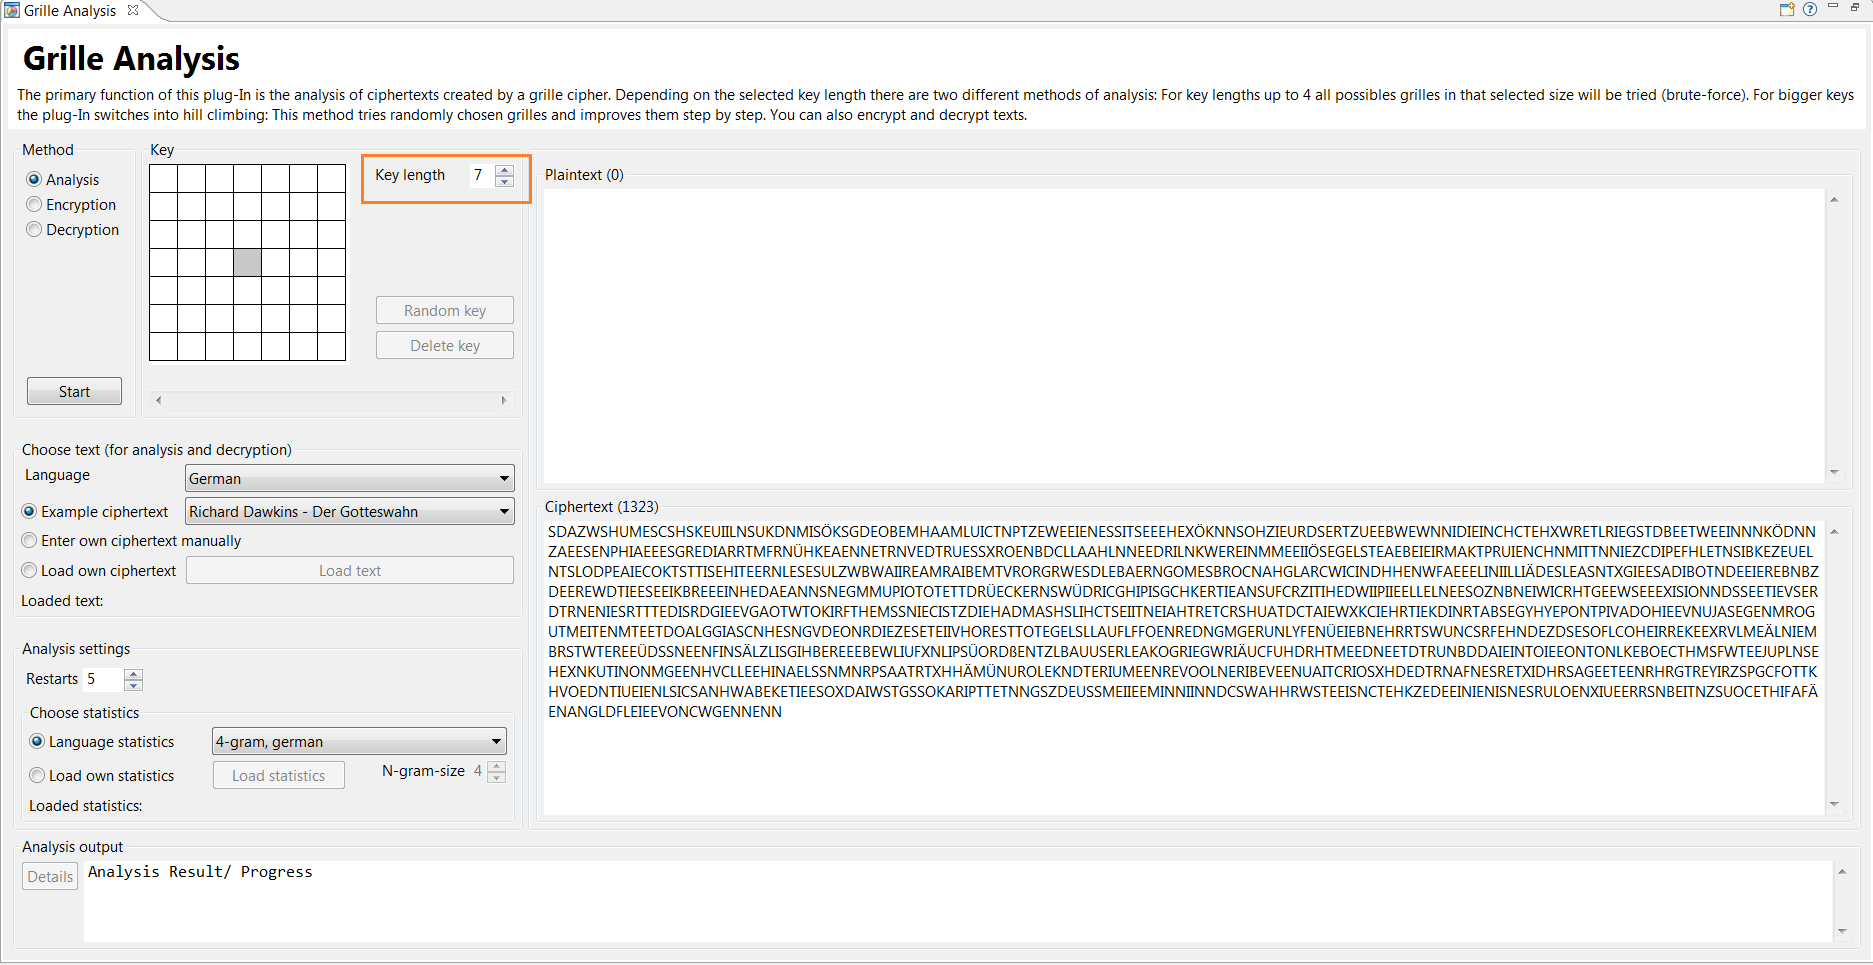
\includegraphics[scale=0.45]{enFleissnerKeySize.png}
For the default setting \glqq Example ciphertext\grqq{} in the section \hyperlink{txtausw}{Choose text} the ciphertext will be adapted to the respective key length. The corresponding key will be randomly generated and discarded after the encryption.

\subsection{Choose text} \hypertarget{txtausw}{}
\subsubsection{Language}
You can select either \glqq German\grqq{} or \glqq English\grqq{} as language. The ciphertext displayed by selecting the option \glqq Example ciphertext\grqq{} (default) -- below the language selection in the section \hyperlink{txteing}{Text input} -- will be updated according to the choosen language.

If a ciphertext is typed in manually or loaded, the language must be adjusted accordingly. Since the analysis is based on language-specific occurences of alphabetic strings, the text being analyzed must be compatible with the selected language.


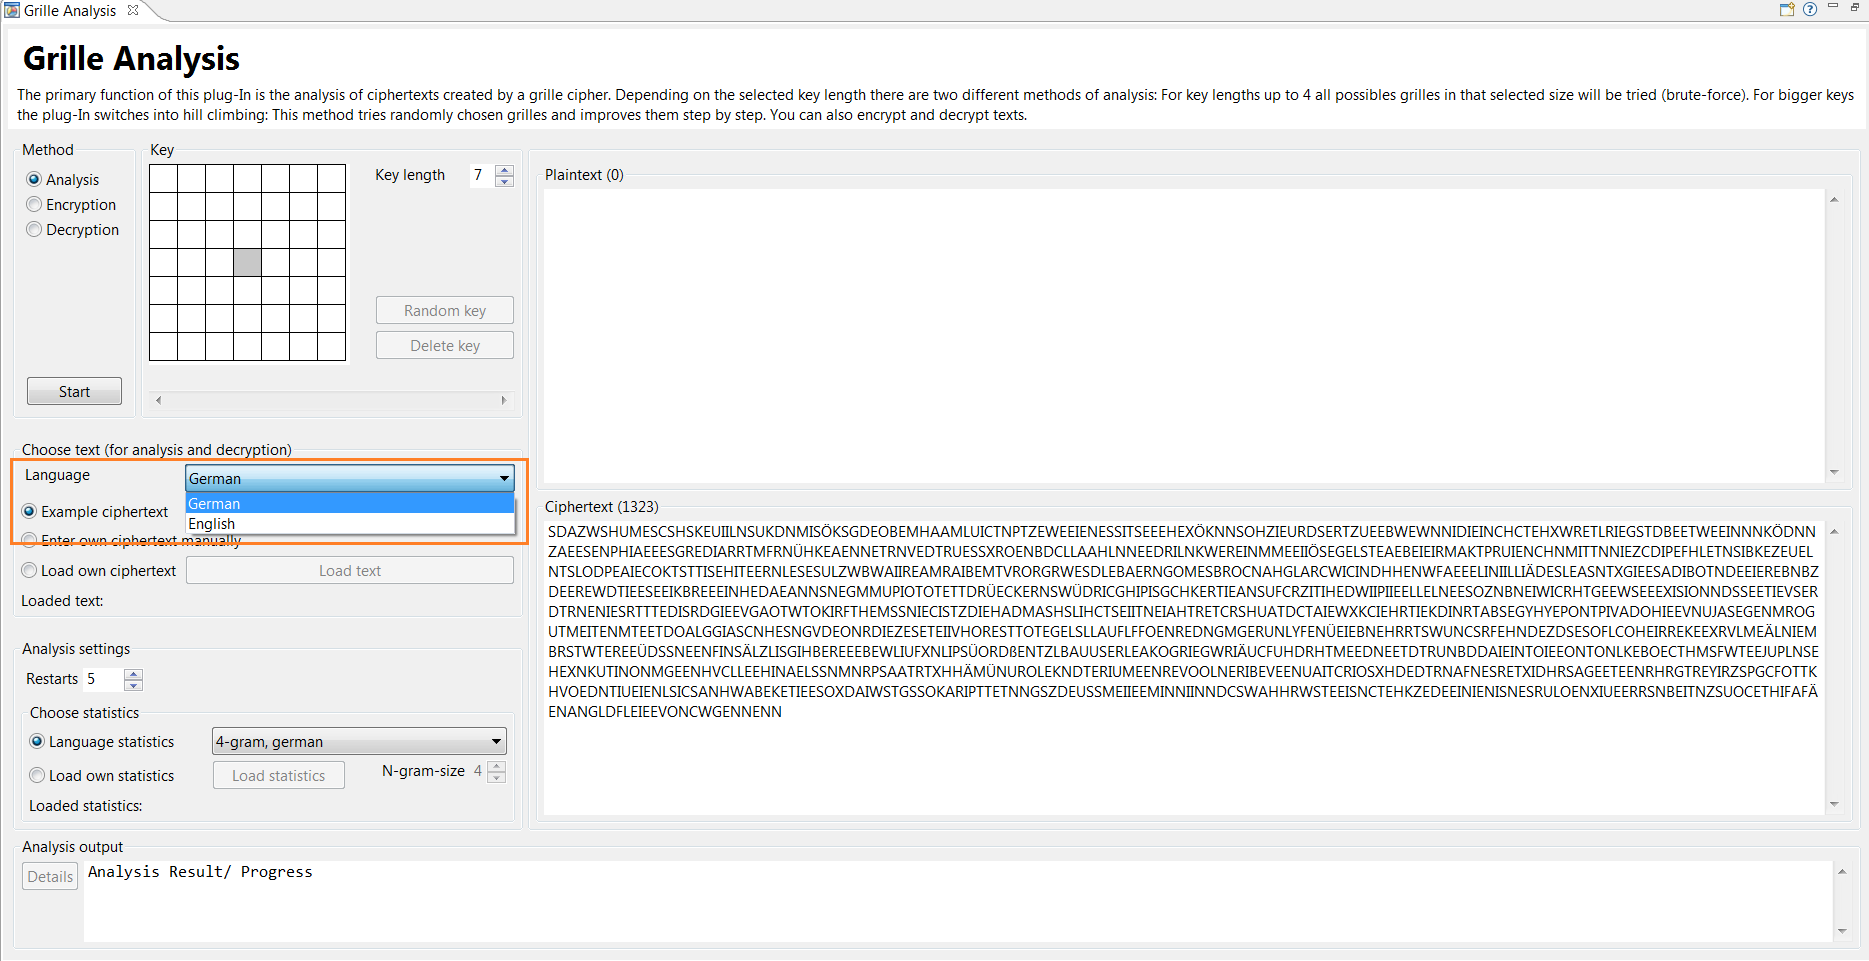
\includegraphics[scale=0.45]{enFleissnerLanguage.png}
\newpage


\subsubsection{Text input}\hypertarget{txteing}{}
In this aggregation the type of text input can be selected. 

\begin{enumerate}[label=(\alph*), leftmargin=*]
\item \textbf{Example ciphertext}

The selection \glqq Example ciphertext\grqq{} is choosen by default. There are two german and two english ciphertexts available for selection. \footnote{\textbf{Sources:}\\ Richard Dawkins - Der Gotteswahn\\ Richard Dawkins - The God Delusion\\ \url{https://de.wikipedia.org/wiki/Bildende_Kunst\#Fr\%C3\%BChchristliche_und_byzantinische_Kunst}\\ \url{https://en.wikipedia.org/wiki/Visual_arts}}

The text encryption will be consistent with the current key length. 

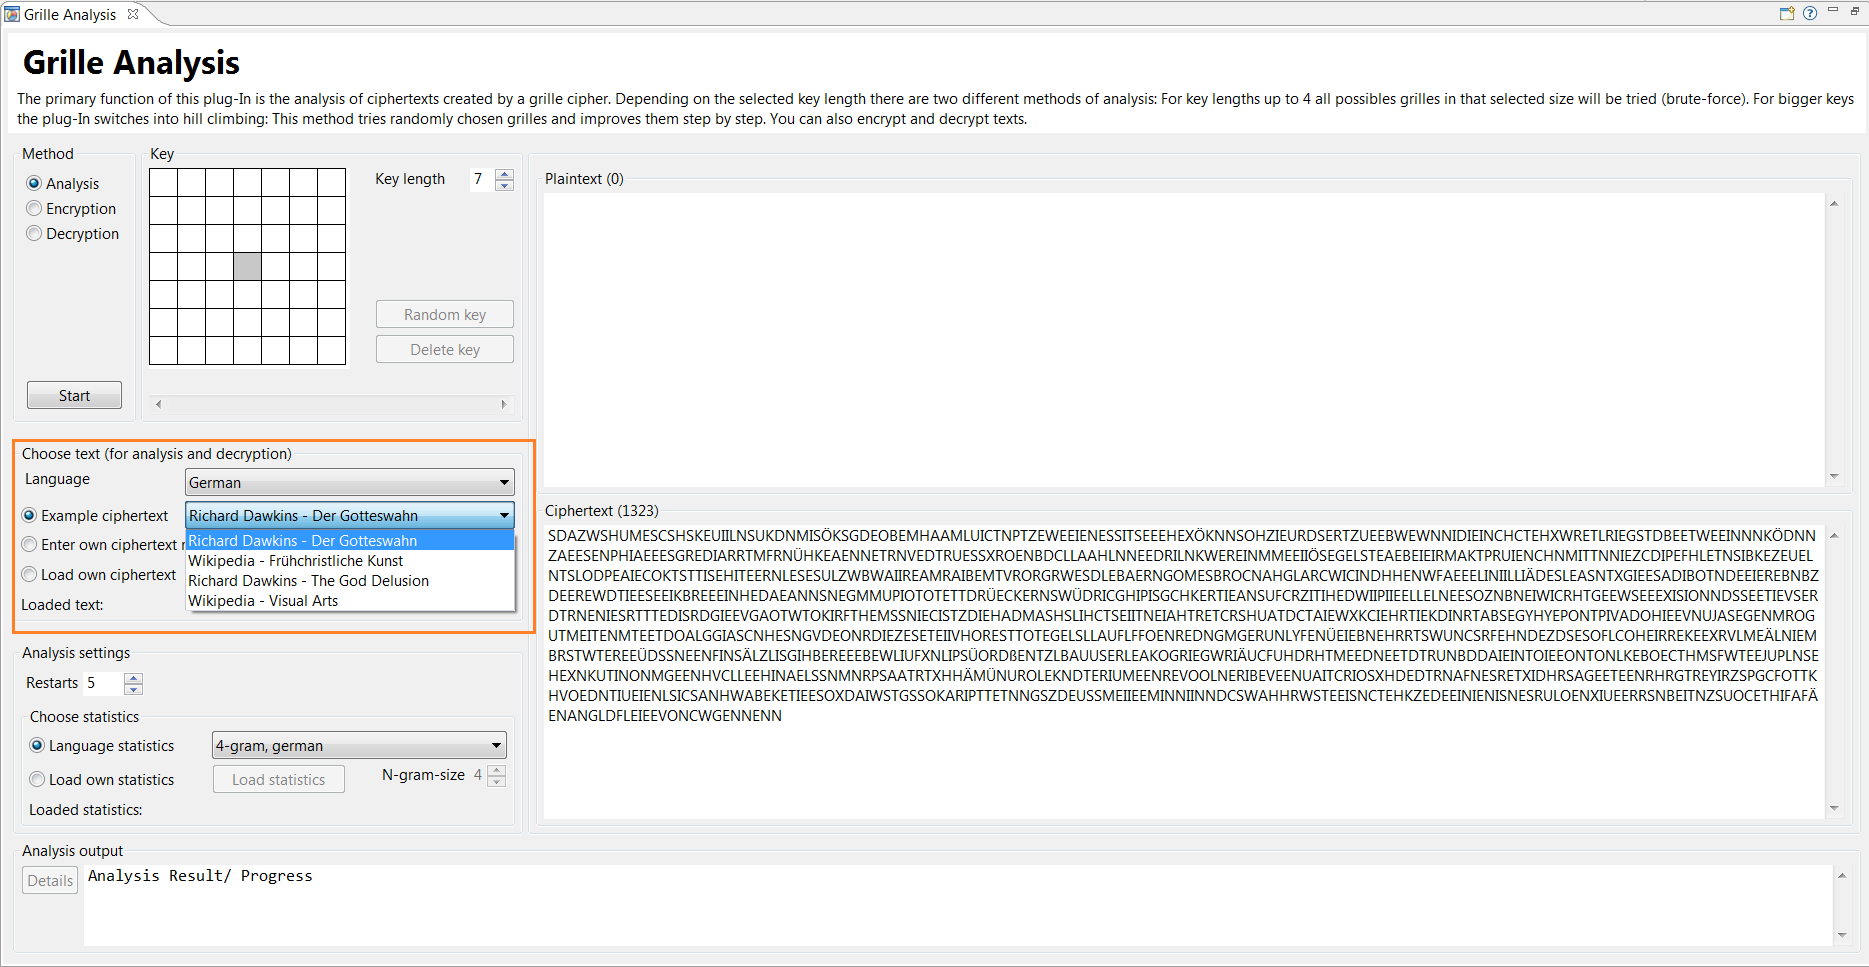
\includegraphics[scale=0.4]{enFleissnerTxtAuswahl.png}
\newpage

\item \textbf{Enter own ciphertext manually}

By selecting the \glqq Enter own ciphertext manually\grqq{} option, the ciphertext field on the right will be available for entering a text.

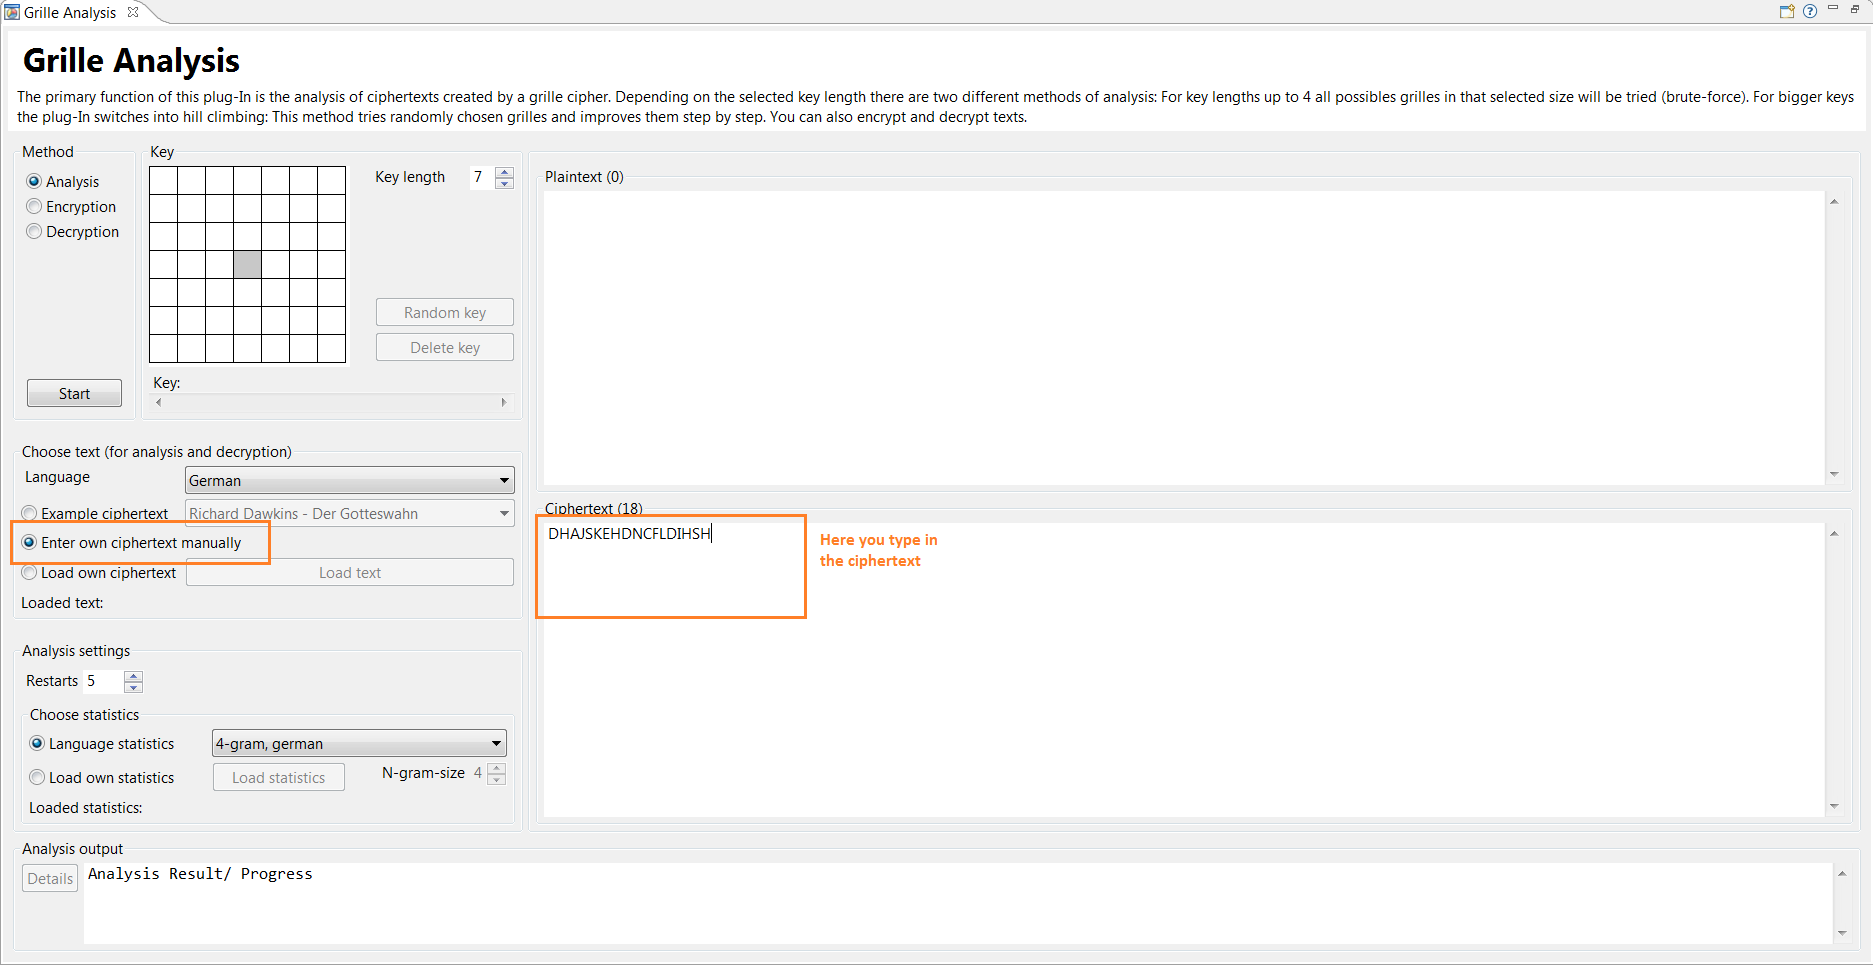
\includegraphics[scale=0.4]{enFleissnerManGhtxt.png}

\item \textbf{Load own ciphertext}

The last selection \glqq Load own ciphertext \grqq{} is available for loading a ciphertext from a file. With this selection the button \glqq Load text \grqq{} is activated which can then be used to load a text file (*.txt). The text is then displayed in the ciphertext field.

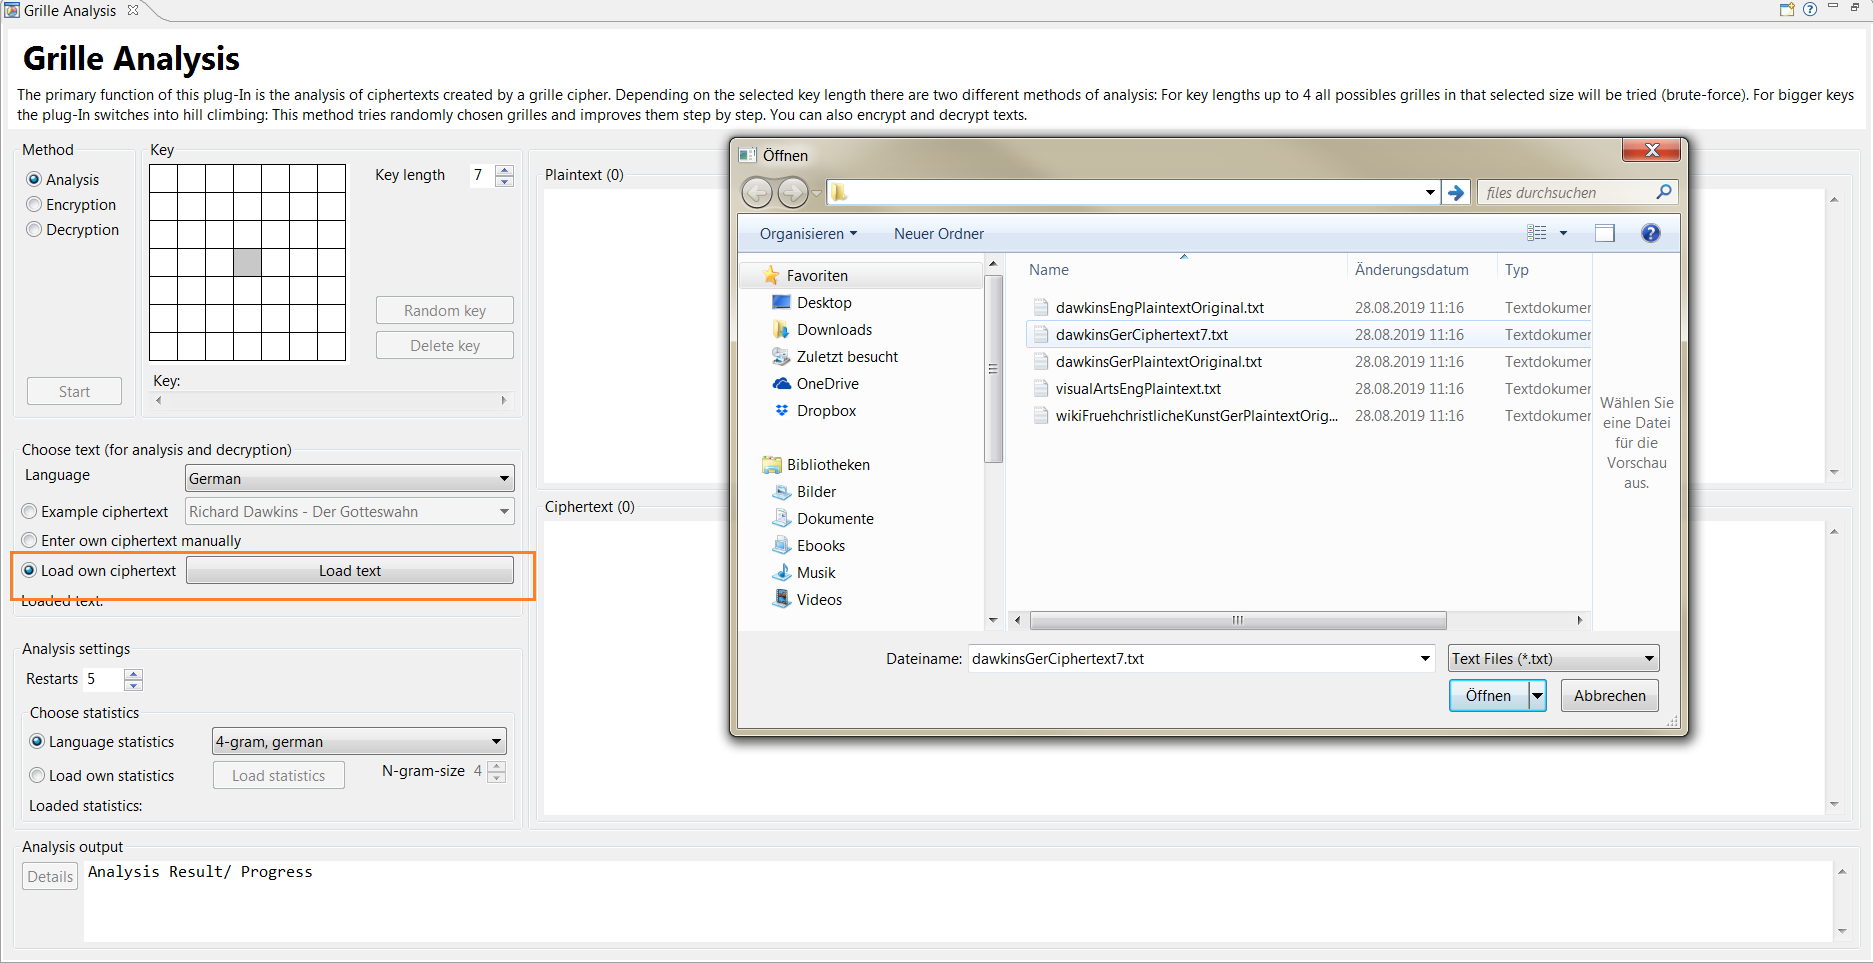
\includegraphics[scale=0.4]{enFleissnerCipherLoadOwn.png}
\end{enumerate} 


\subsection{Analysis settings}
The \glqq Analysis settings\grqq{} section is located directly below the \glqq \hyperlink{txtausw}{Choose text}\grqq{} section and is only activated for the analysis function.

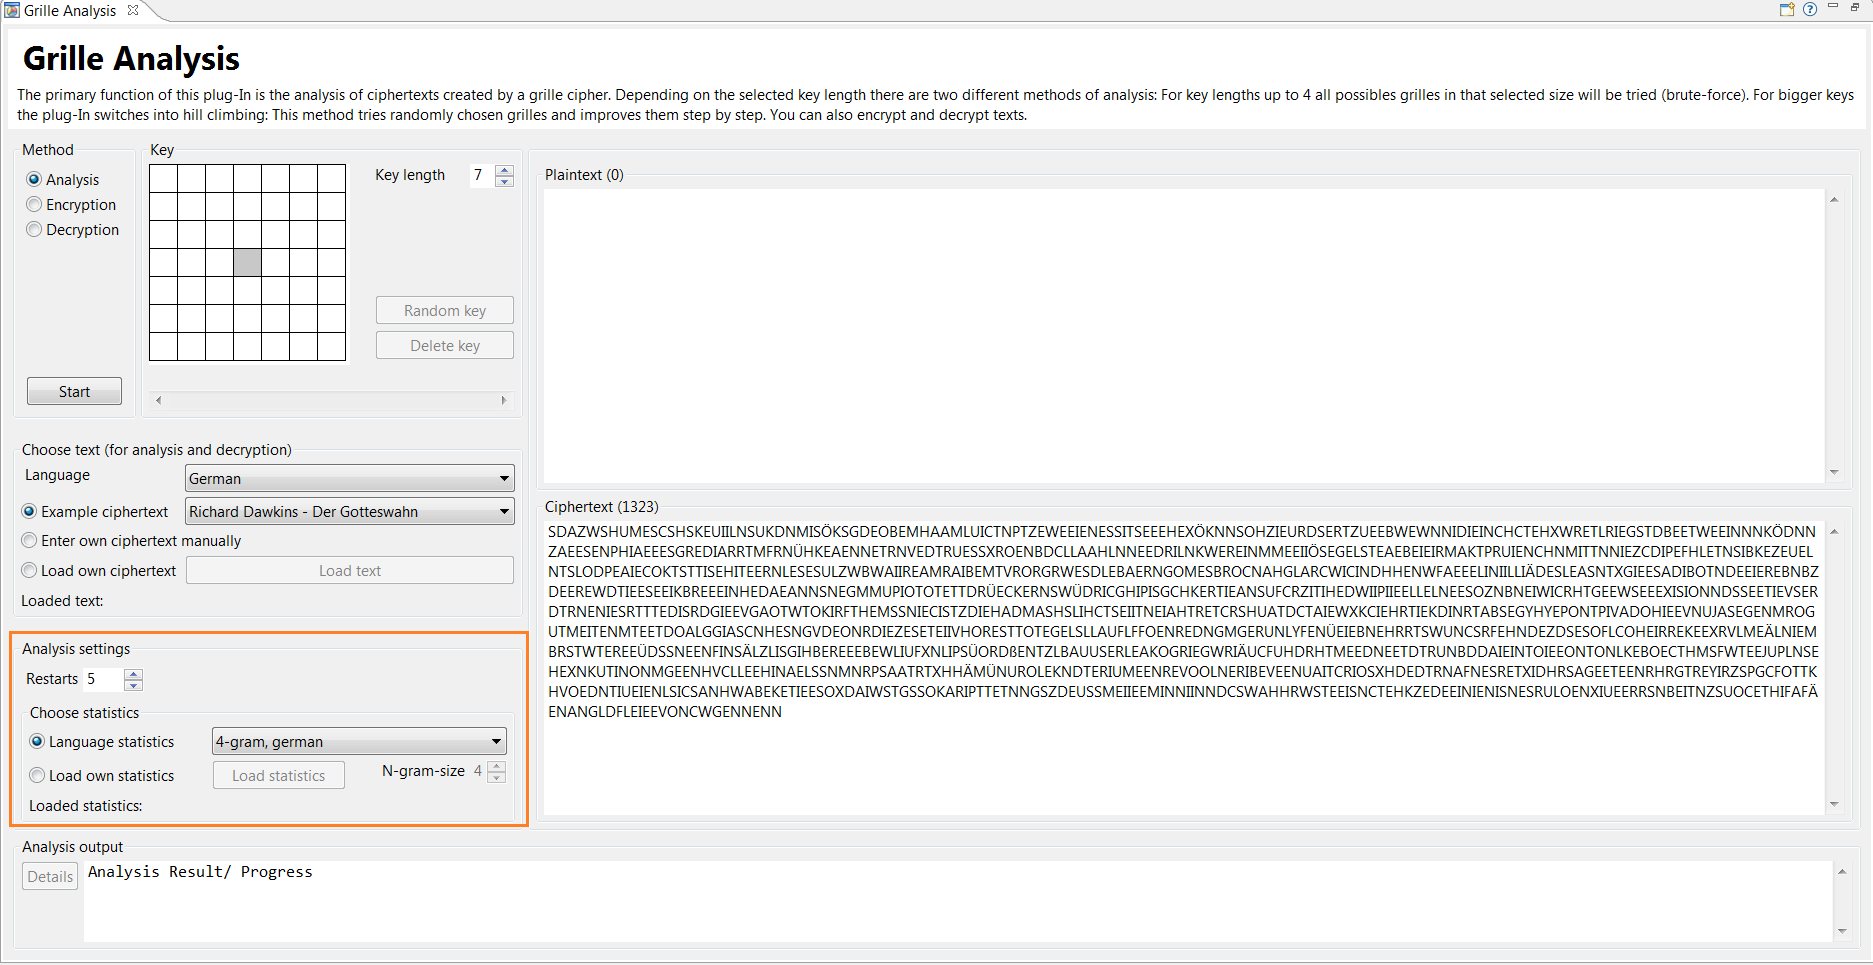
\includegraphics[scale=0.45]{enFleissnerAnalysisSettings.png}


\subsubsection{Restarts}
The number of \glqq restarts\grqq{} is relevant and thus only enabled for the analysis of ciphertexts that were encryped with a key of size 5 or higher. For a key length with the aforementioned size a \glqq hill climbing\grqq- algorithm will be implemented for the analysis. Every restart creates a new random key for the selected key size. This respective key is then improved step by step by only changing one hole at a time and comparing the quality of the resulting decrypted text. Every improvement is saved and then used as the basis for the next improvement search. This pattern will be repeated until no further improvements can be made by changing one hole.
The higher the number of restarts, the higher the chance of finding the right key through the analysis will be.

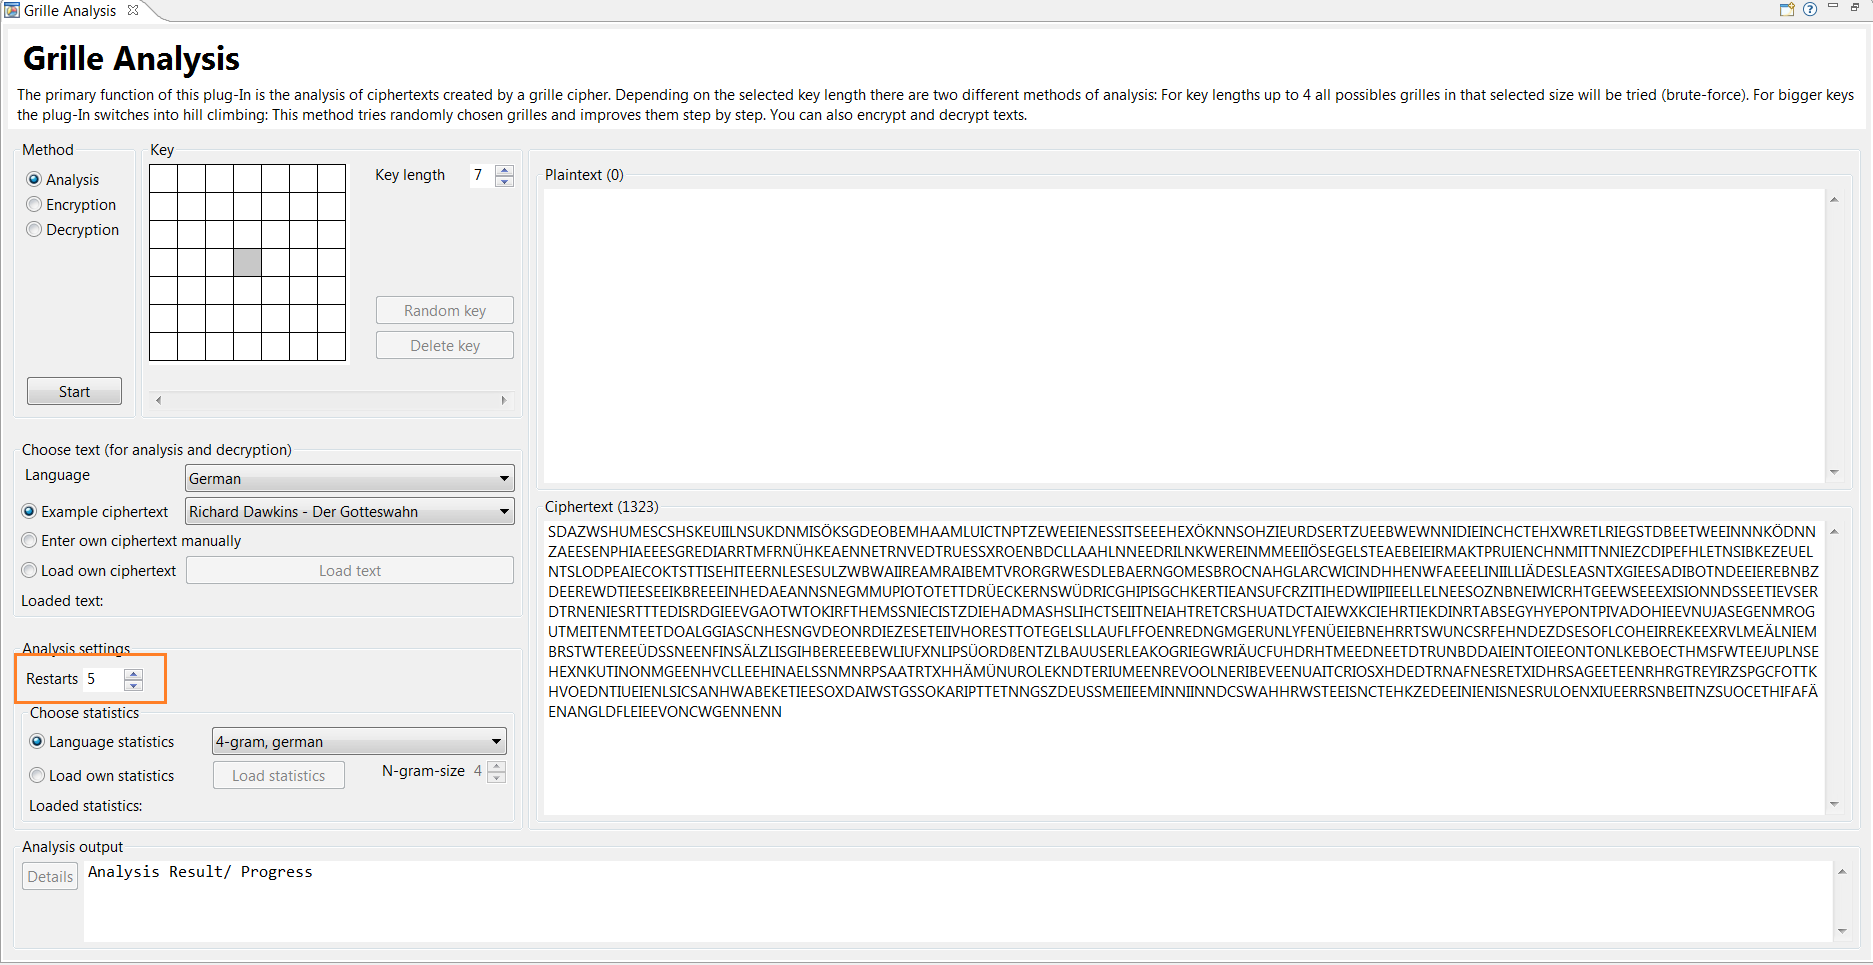
\includegraphics[scale=0.45]{enFleissnerRestarts.png}

\textbf{Note:} Expect a longer processing time for larger keys and a higher number of restarts. \footnote{Appendix: Evaluation of the analysis}

\subsubsection{Language statistics}
The language statistics are essential for the analysis of a ciphertext. It contains the probability of occurrence of all coherent character strings of a certain length $n$ (n-grams) in the respective language. The language of the ciphertext must agree with the selected or loaded statistics. Otherwise, the probability of success drops considerably.

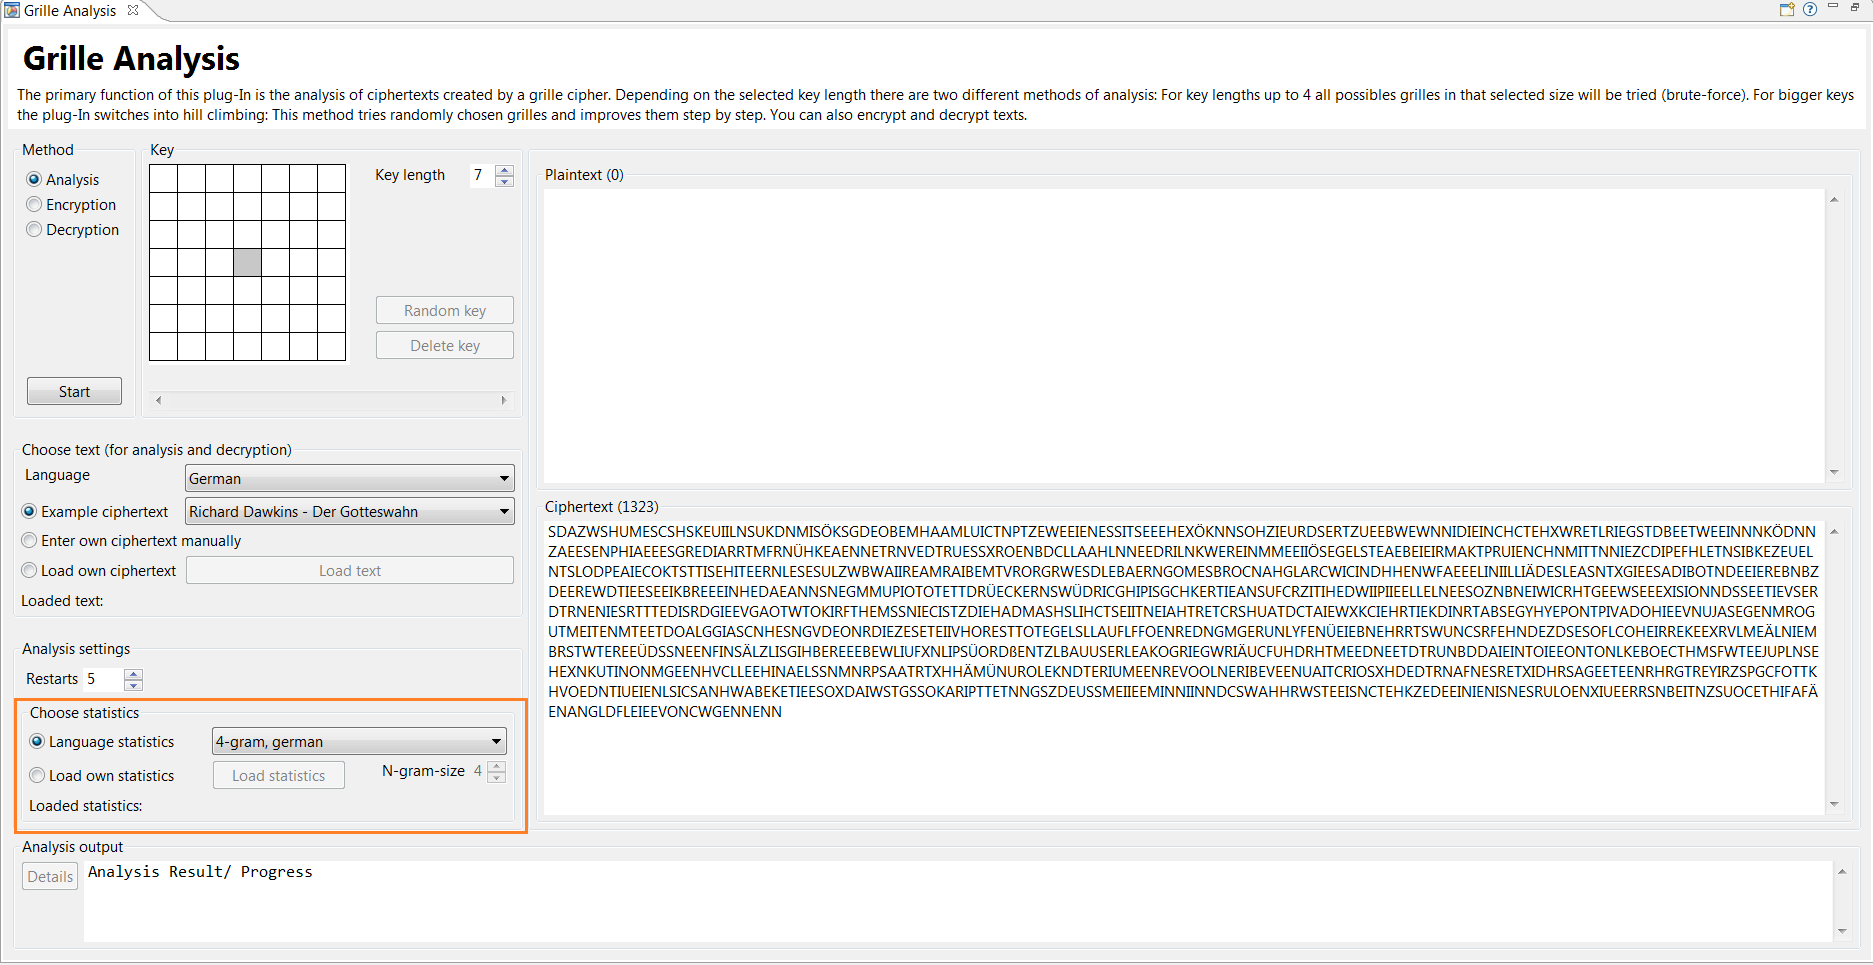
\includegraphics[scale=0.45]{enFleissnerStatistics.png}

\begin{enumerate}[label=(\alph*), leftmargin=*]
\item \textbf{Language statistics}

To carry out the analysis, one of the three stored statistics can be applied (one in german and two in english).

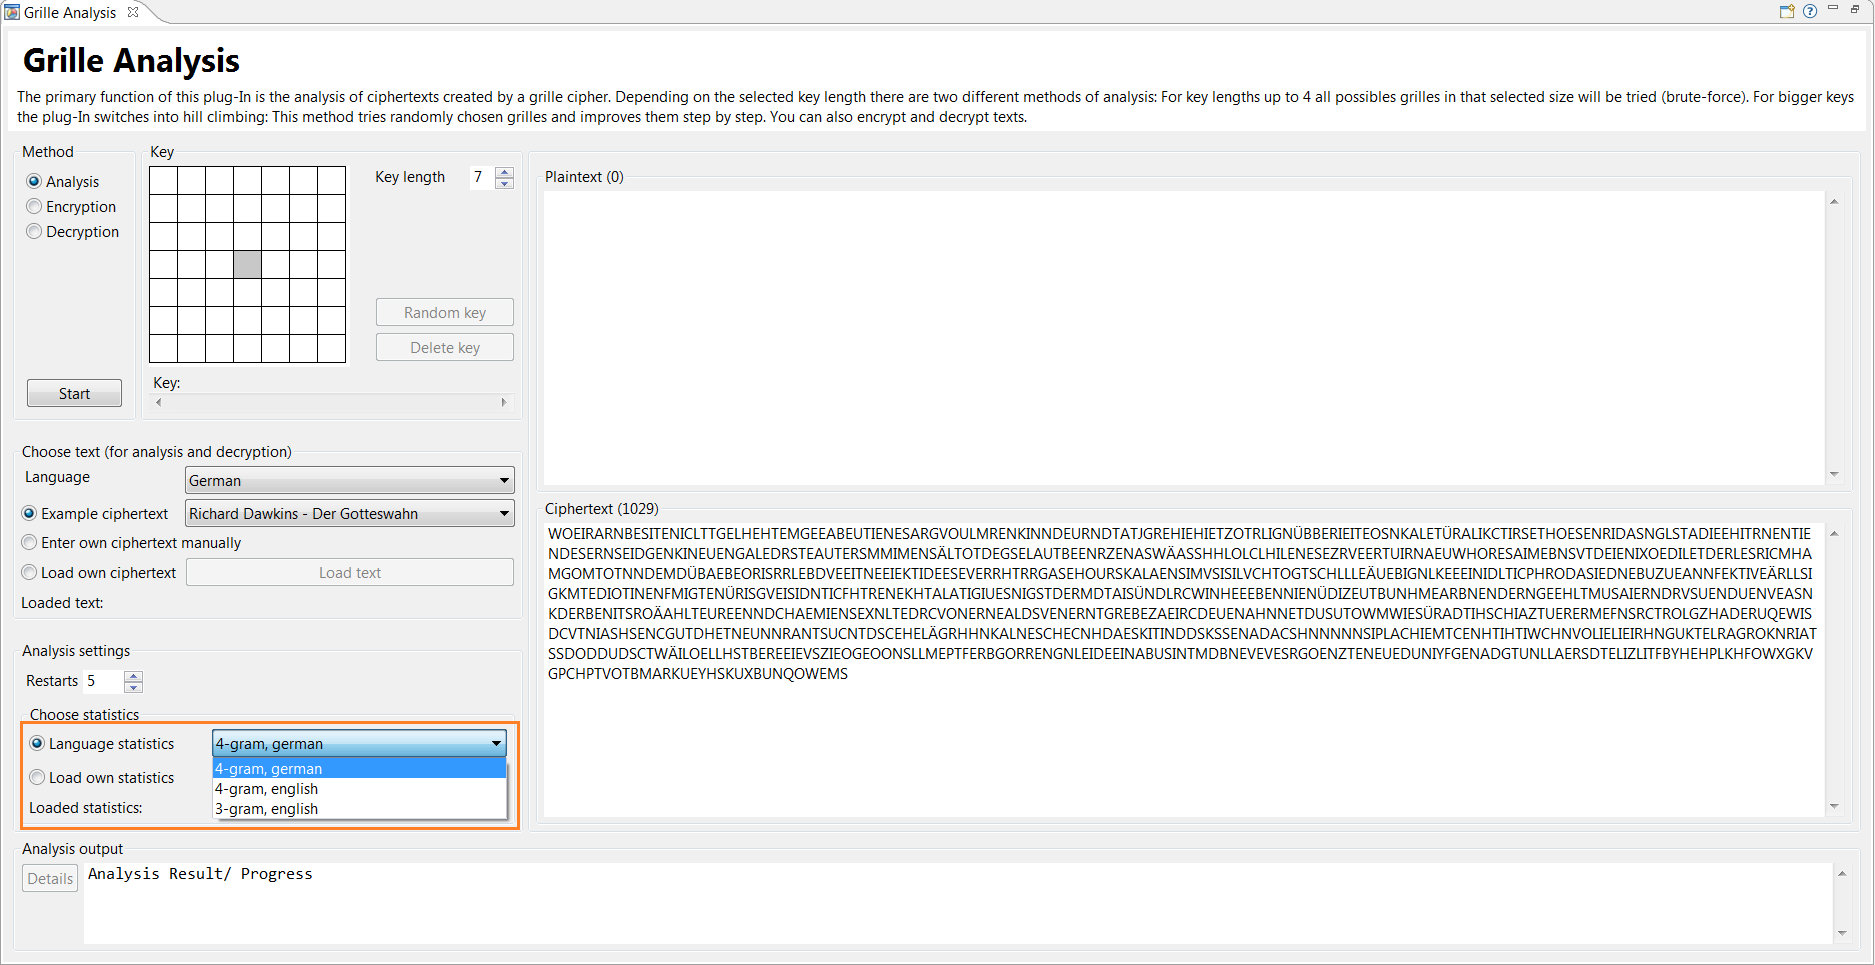
\includegraphics[scale=0.4]{enFleissnerStatisticsExample.png}


\item \textbf{Load own statistics}

The option to load language statistics files is also available. The following are \textit{requirements} for the format of a usable language statistics: Compared to other language statistics, the actual n-grams for this plug-in should not be in the file. The language statistics used should only contain the logarithmized values of the respective n-grams. For this purpose, the language statistics are built up like an $n$ -dimensional cube, where the position of the letters in the alphabet and the position of each letter in the n-gram together form the index for the value of the respective n-gram.


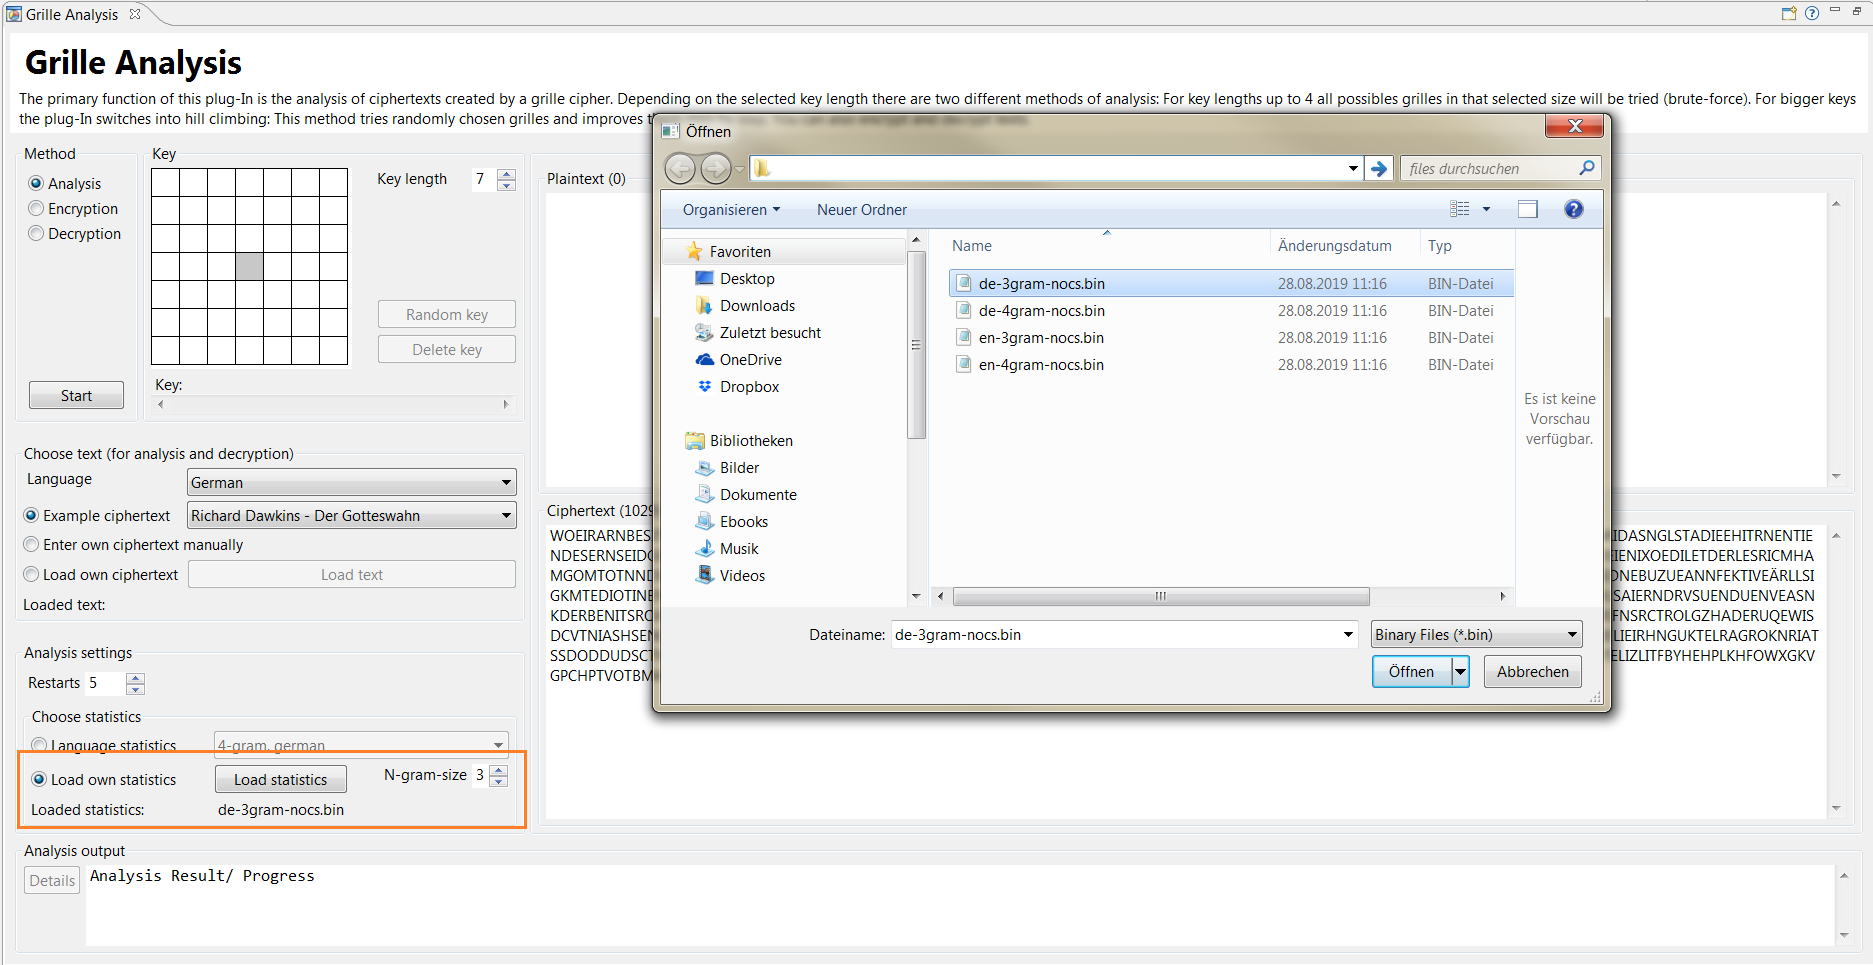
\includegraphics[scale=0.4]{enFleissnerOwnStatistics.png}

\textbf{Example:}
To save and retrieve the quadgram \glqq This\grqq{} in an english quadgram statistic, proceed as follows (with lower case letters being treated like upper case letters):

The english alphabet is given  in the form \glqq ABC ... XYZ\grqq{} of length 26, whereby each letter is assigned an index from $ 0 $ to $ 25 $. For the quadgram \glqq This\grqq, each letter index of the quadgram is now multiplied by a power of the alphabet length depending on the position in the quadgram. These four values are summed together resulting with the index of the quadgram value in the language statistics. As mentioned above, the letters T, h, i, and s are each assigned the index 19, 7, 8, and 18. The calculation mentioned above

\[
19*26^3+7*26^2+8*26^1+18*26^0=19*17576+7*676+8*26+18=338,902
\]

for the index of the quadgram \glqq This\grqq{} in an english quadgram statistic can now be carried out.

Loading customized language statistics requires manual entry of the size of the n-grams in this aggregation \glqq Choose statistics\grqq .
\end{enumerate}
\newpage

\subsection{Analysis output}

The analysis output window is located at the bottom of the screen. The selected parameters are displayed at the start of the analysis. After completing the analysis, additional information such as the key found, the resulting plaintext, and the time required for the run are displayed. 

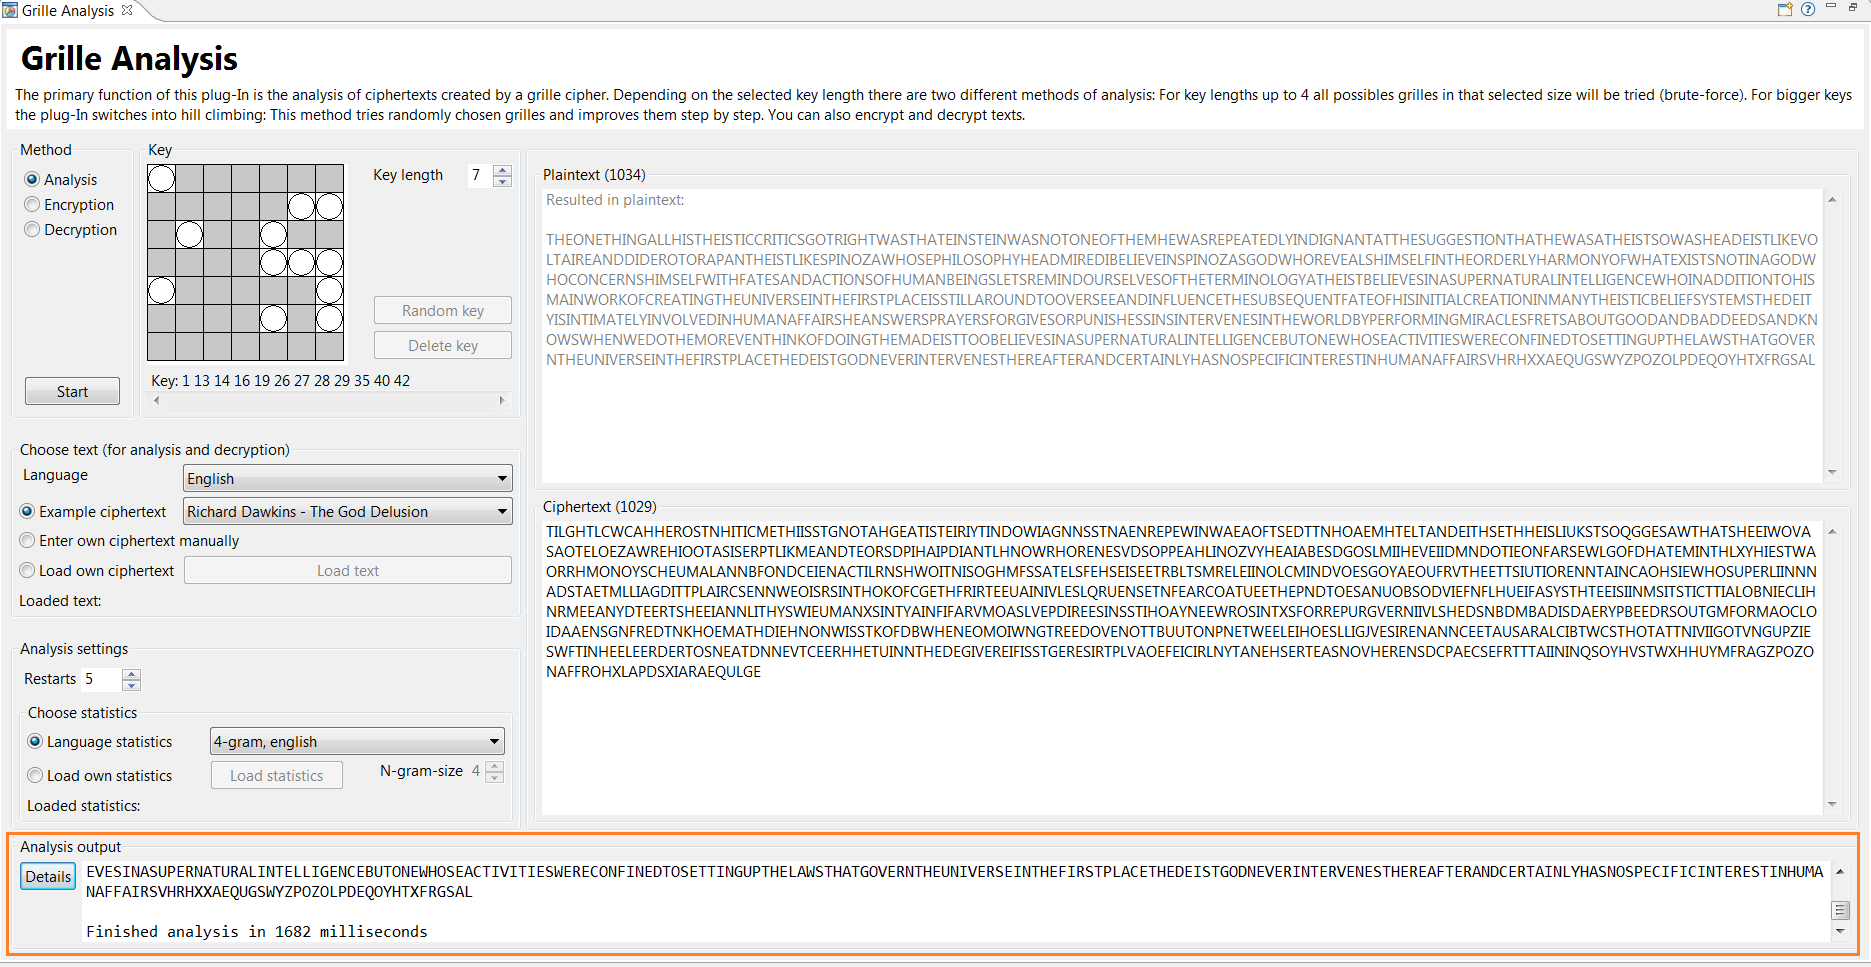
\includegraphics[scale=0.45]{enFleissnerAusgabeAnalyse.png}

The \glqq Details\grqq{} button on the lefthand side of the output field provides additional information.

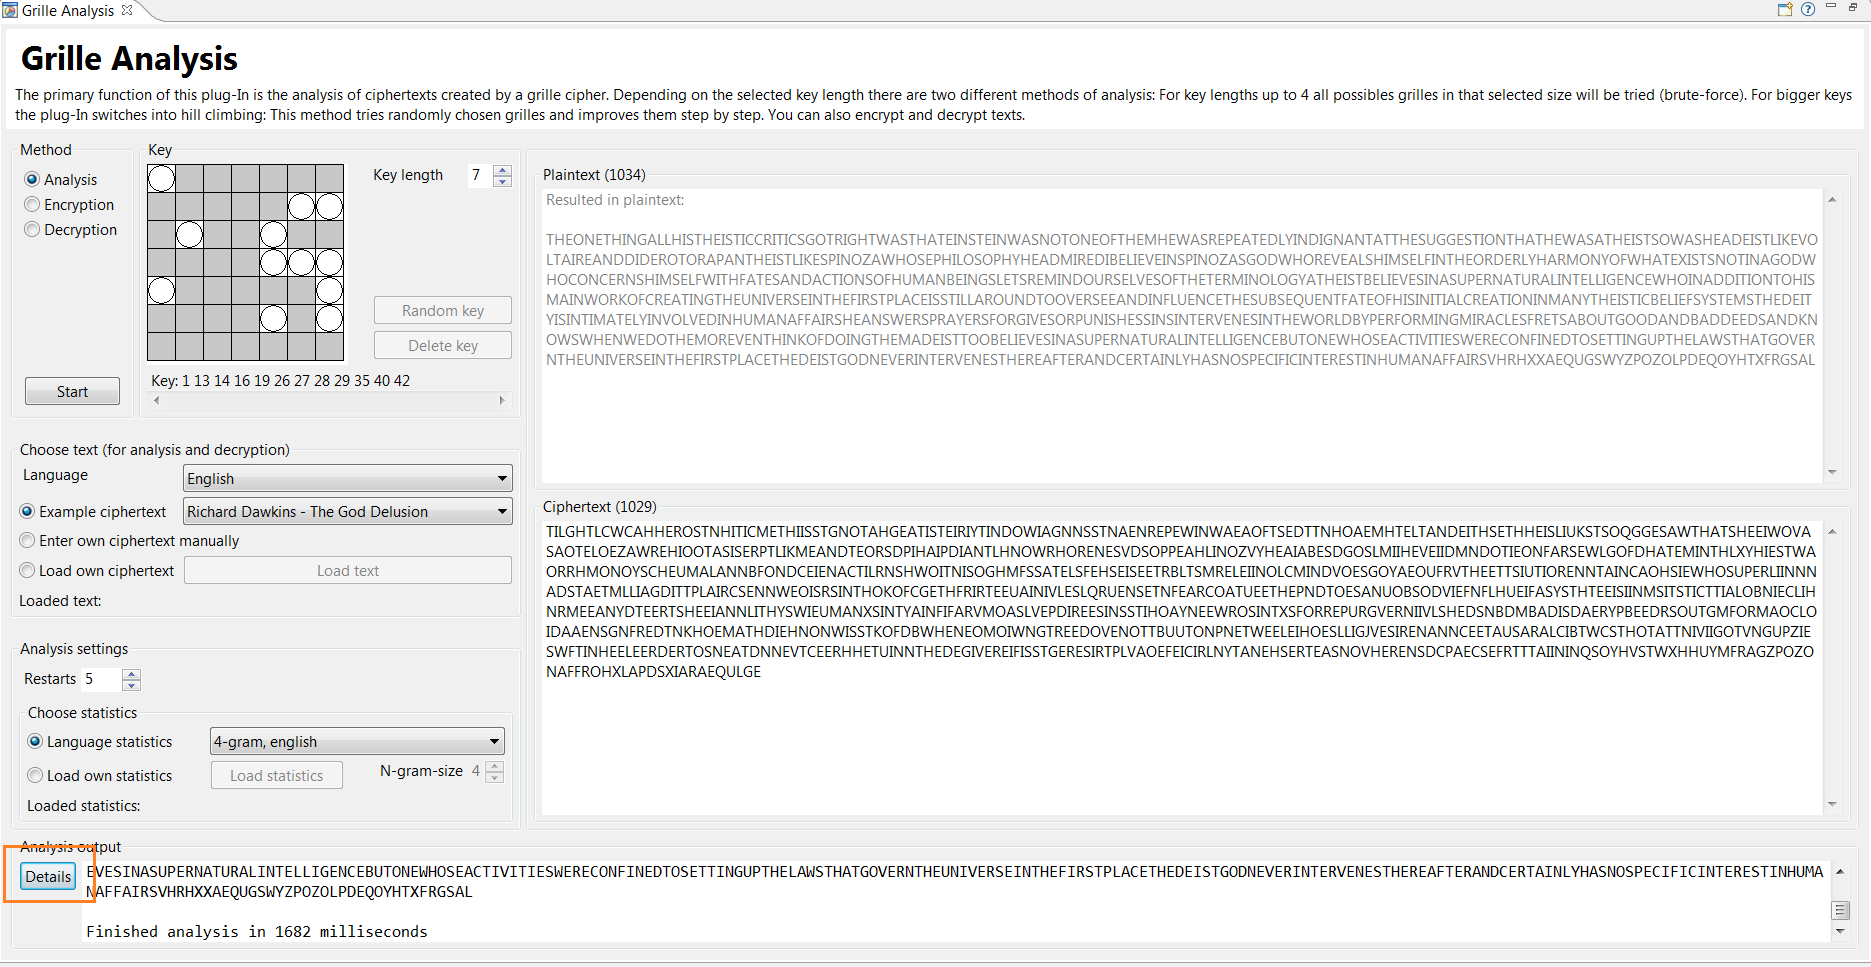
\includegraphics[scale=0.45]{enFleissnerAusgabeAnalyseDetailButton.png}

This opens a new dialog window in which information from the output window and intermediate outputs from the analysis process are displayed. This output can then be saved as a text file (*.txt).

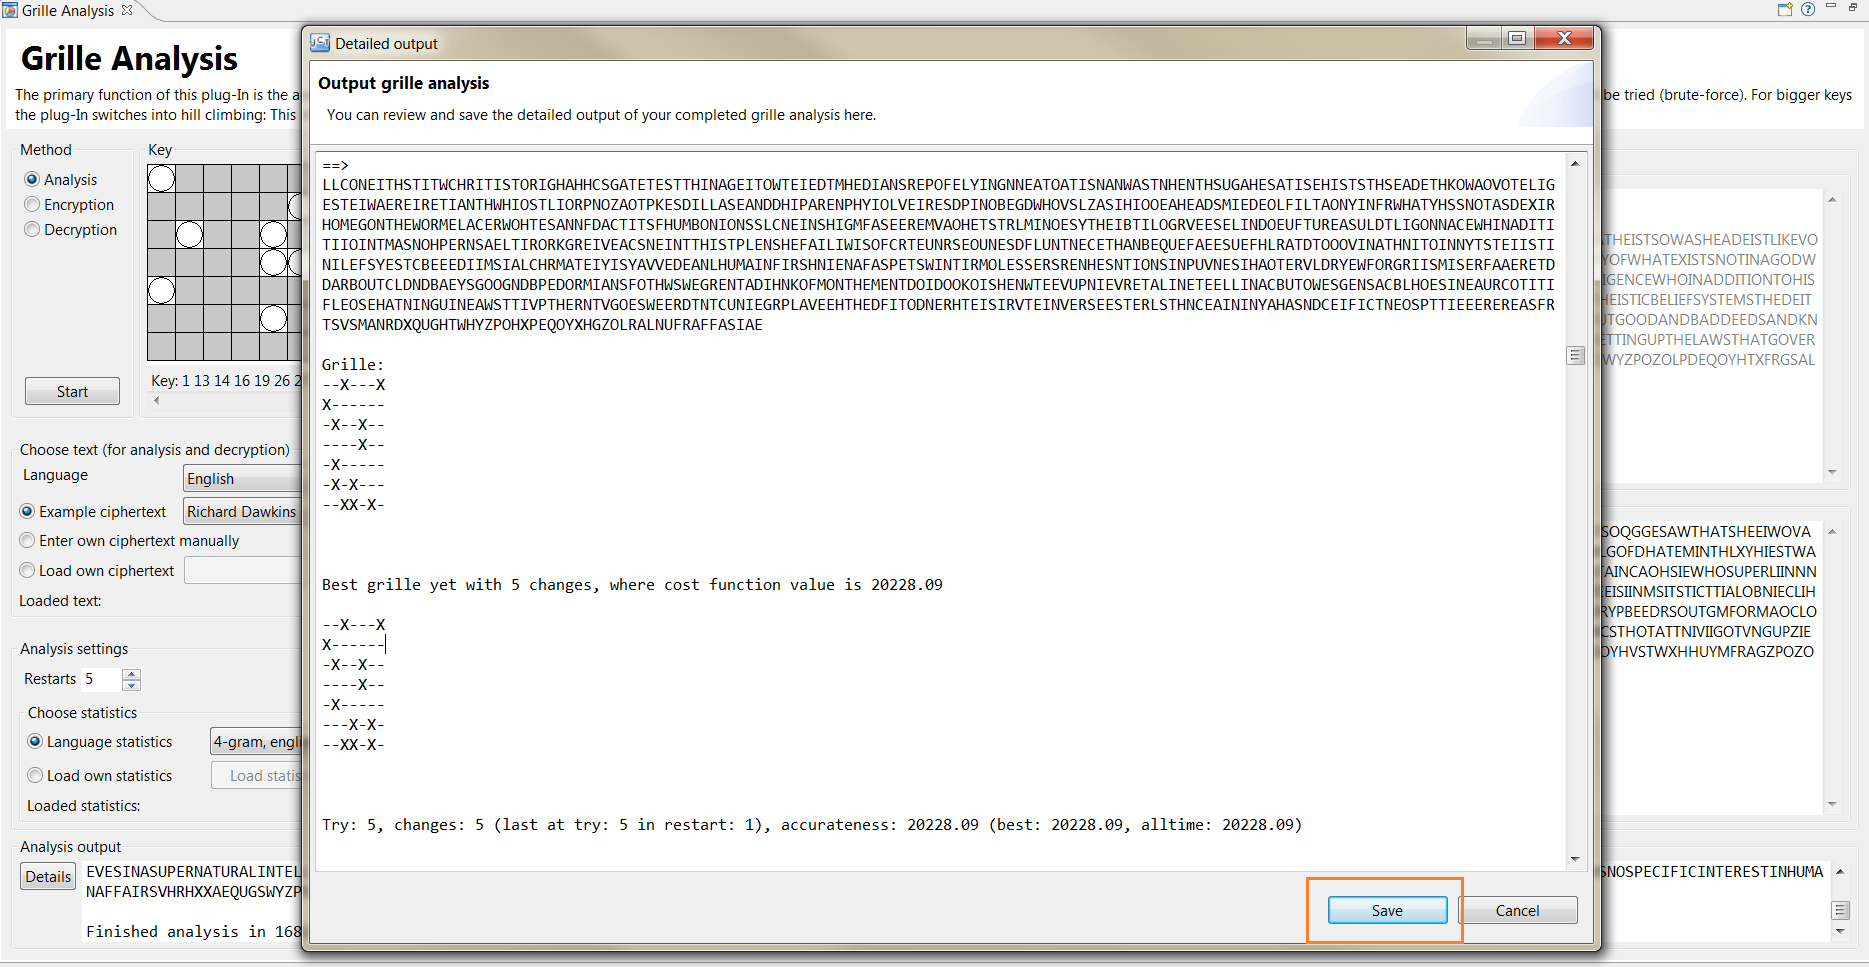
\includegraphics[scale=0.45]{enFleissnerAusgabeAnalyseGross.png}

After completition of the analysis, the key found is also displayed in the key field itself, in order to be applied, for example, directly for decryption and thus validation of the analysis result.
\newpage

\section{Encryption}\hypertarget{verschl}{}
In this plug-in, plaintexts can also be encrypted. For this purpose, select the function \glqq Encryption\grqq{} in the aggregation \glqq Method\grqq{}. This entails that the buttons \glqq Random key\grqq{} and \glqq Delete key\grqq{} will be enabled (in case, analysis is selected, both buttons are disabled).


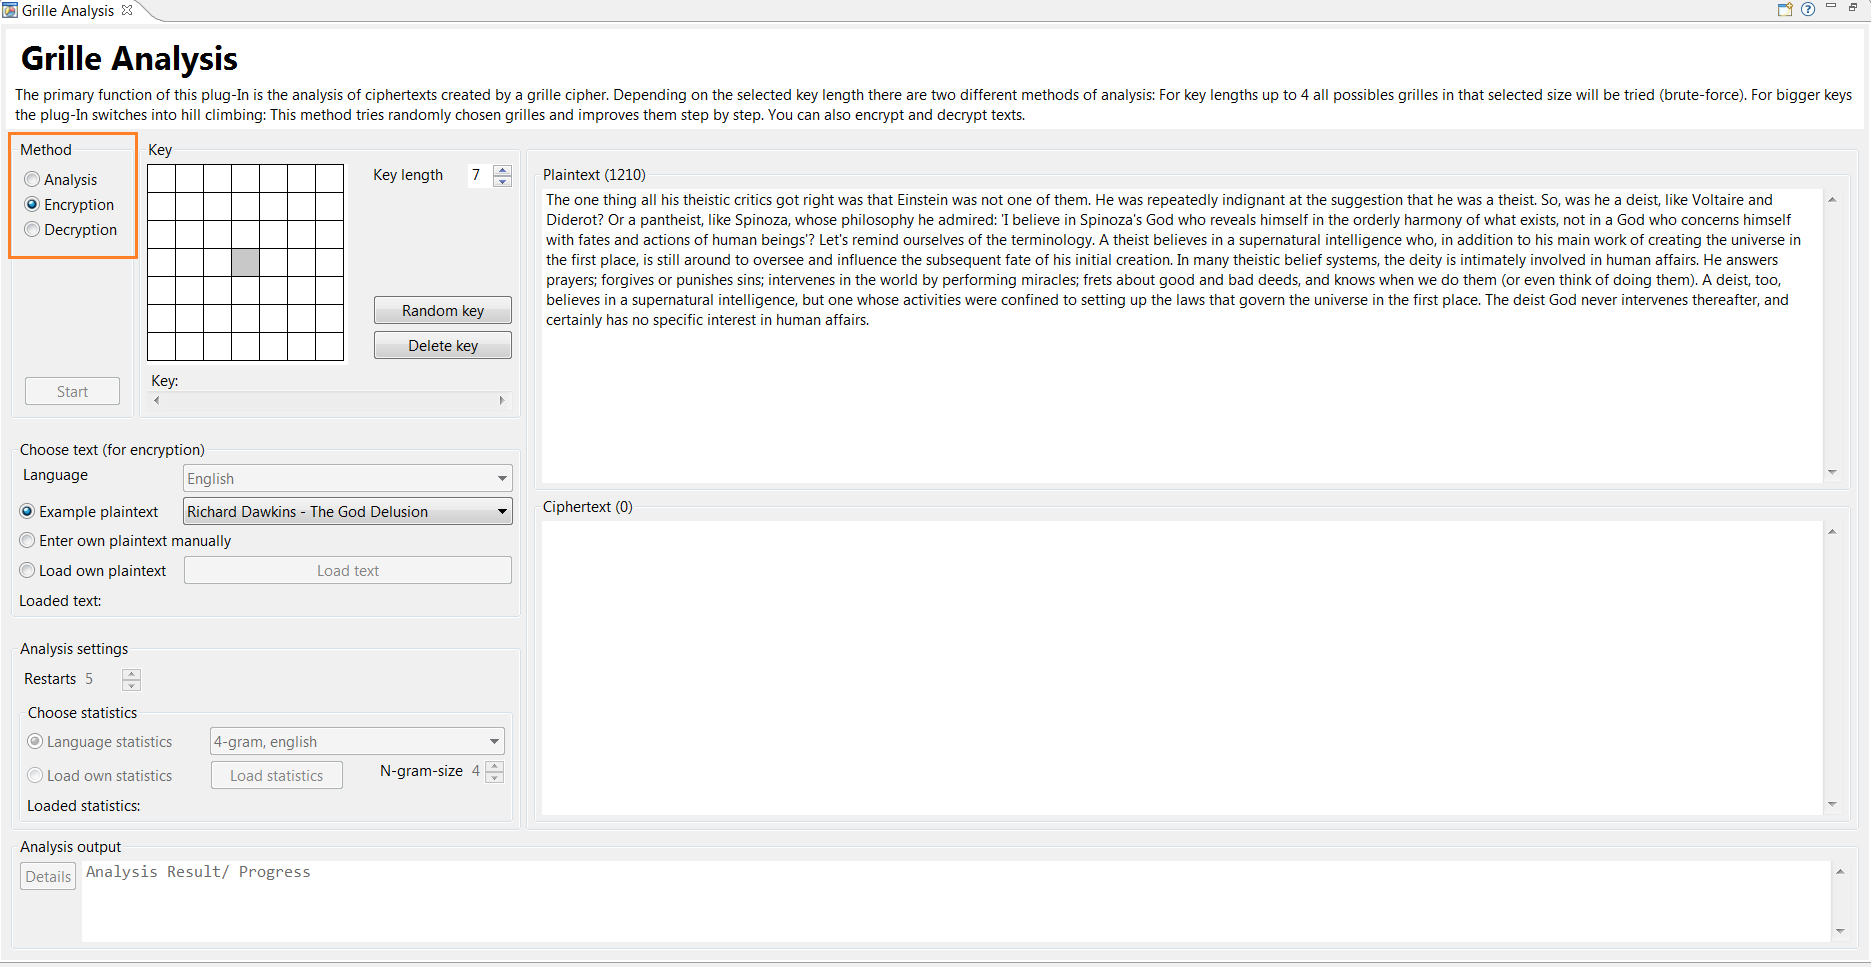
\includegraphics[scale=0.45]{enFleissnerEncryptSelection.png}


\begin{enumerate}[label=(\alph*), leftmargin=*]
\item \textbf{Random key}

By pressing the button \glqq Random key\grqq{} a random key is generated and displayed. 

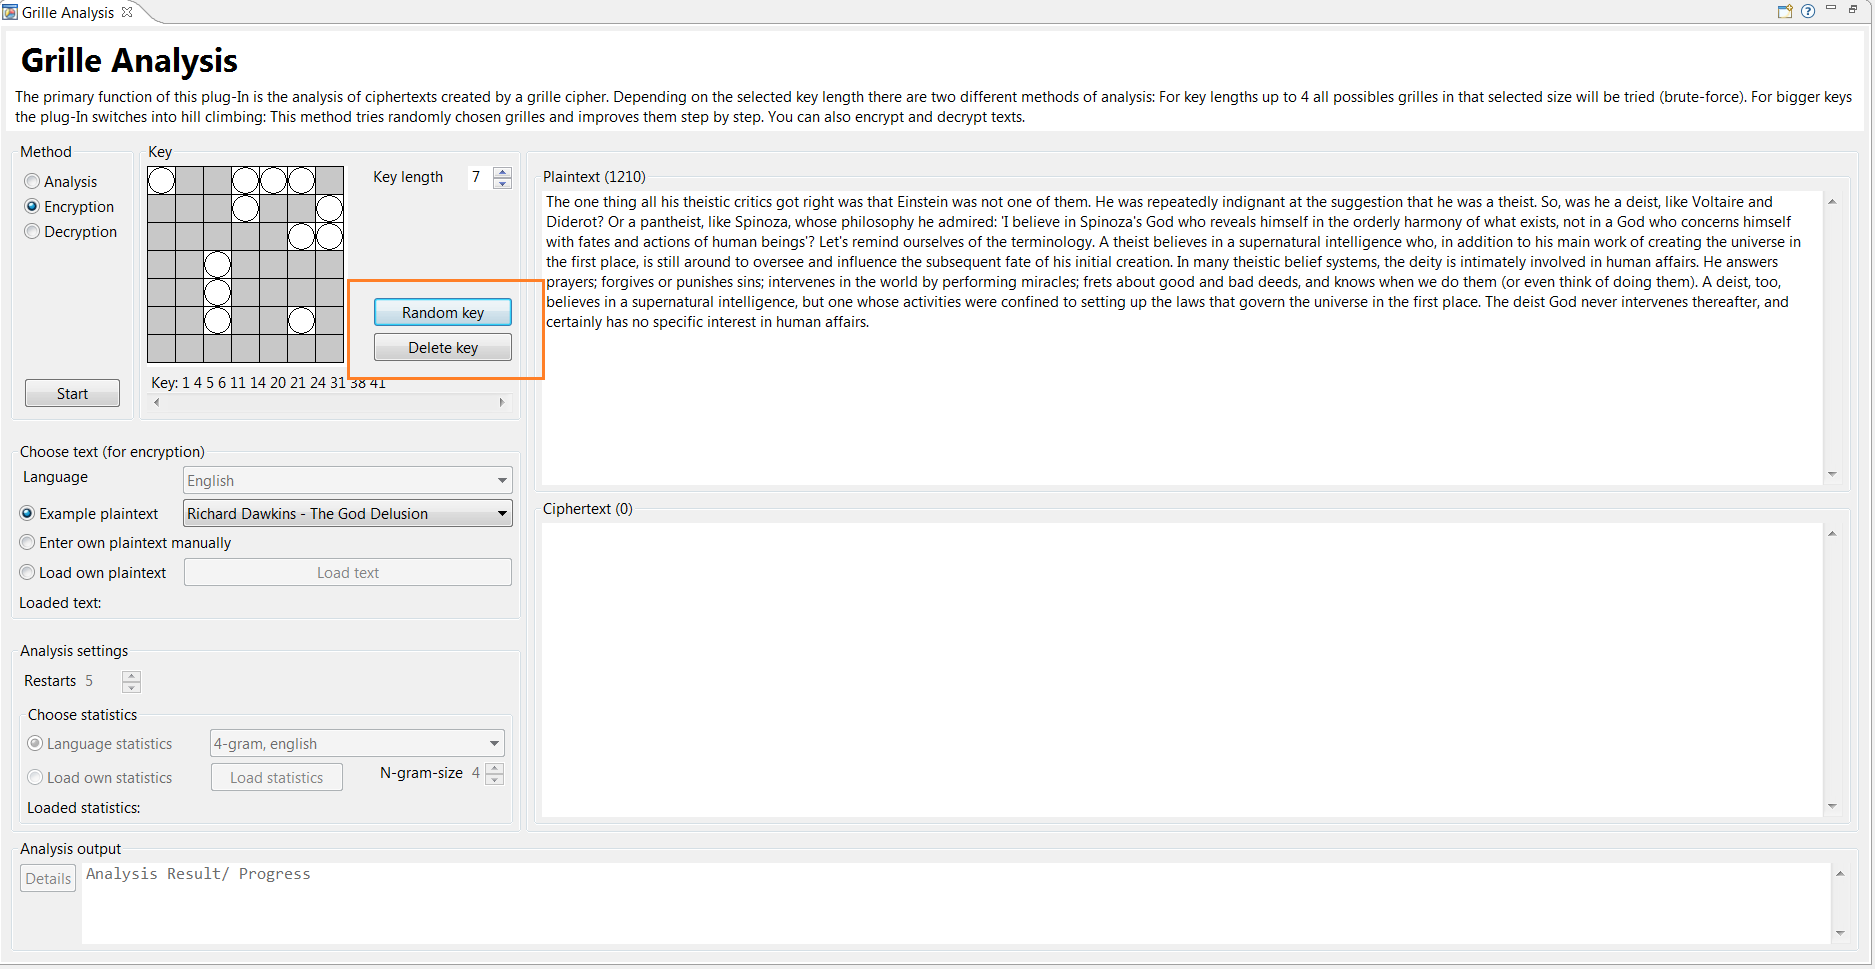
\includegraphics[scale=0.4]{enFleissnerEncryptRandomKey.png}
\newpage

\item \textbf{Creating a key manually}

To create a key manually, select the fields in which the template should contain the holes for entering the plain text. For each selected field, the three associated fields in the other three quadrants, that are required by the rotation in the encryption process are blocked. If an already selected field is clicked again, the selection of this field is removed.

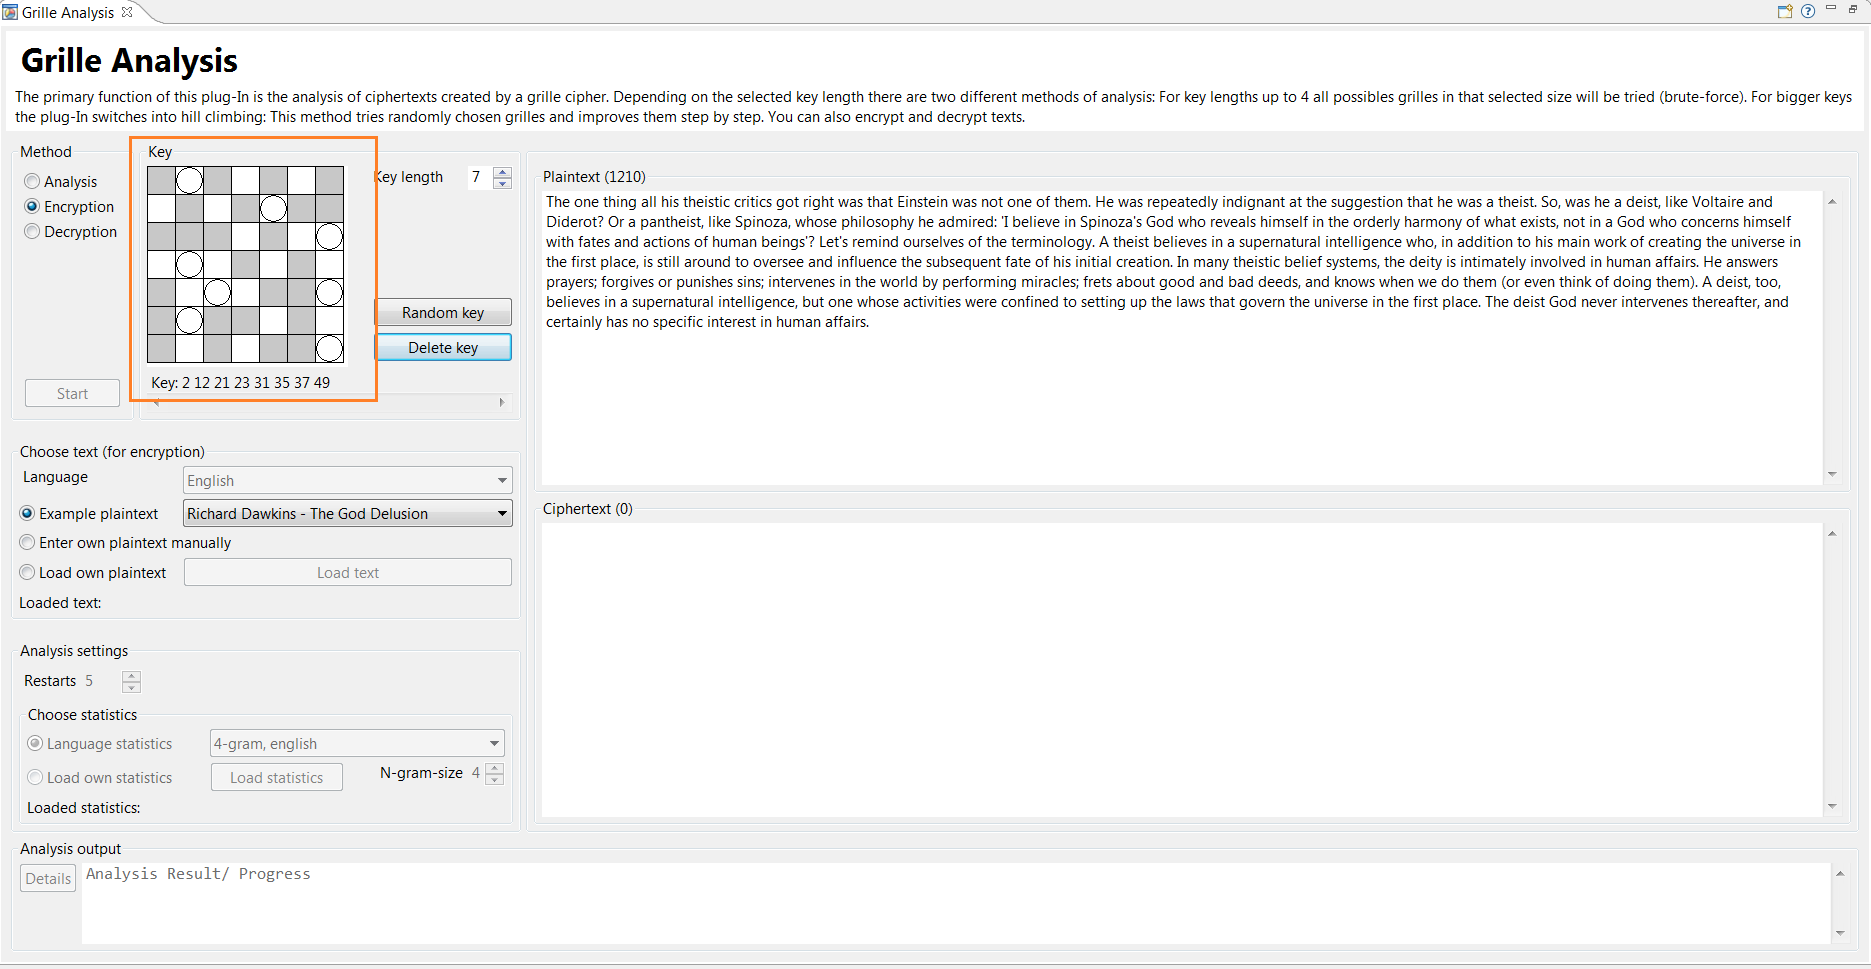
\includegraphics[scale=0.4]{enFleissnerEncryptKeySelection.png}
\end{enumerate} 

Click on the \glqq Delete key\grqq{} button to deselect all fields simultaneously.

The selected holes in the key are also displayed in numerical form under the key field. The fields are numbered from top left to bottom right (starting with 1).

In addition to the key, a plaintext is also required for encryption. As in the analysis function, this can be selected from a number of example texts, typed in, or imported. After selecting example texts, the selected function of the plug-in is recognized and accordingly a plaintext or ciphertext is loaded into the corresponding window. This distinction must be made for manually customized texts, meaning that the plug-in does not recognize whether there is a plaintext or a ciphertext.

If there is a valid key and a text in the plain text field, the \glqq Start\grqq{} button will be activated and the encryption can be carried out.

After changing the method selection to \glqq Analyze\grqq{} or \glqq Decryption\grqq{} continue with the self-generated ciphertext.


\section{Decryption}\hypertarget{entschl}{}

As a final functionality, the plug-in offers decryption, allowing for key implementation obtained from an analysis as well as ciphertext decryption.
 

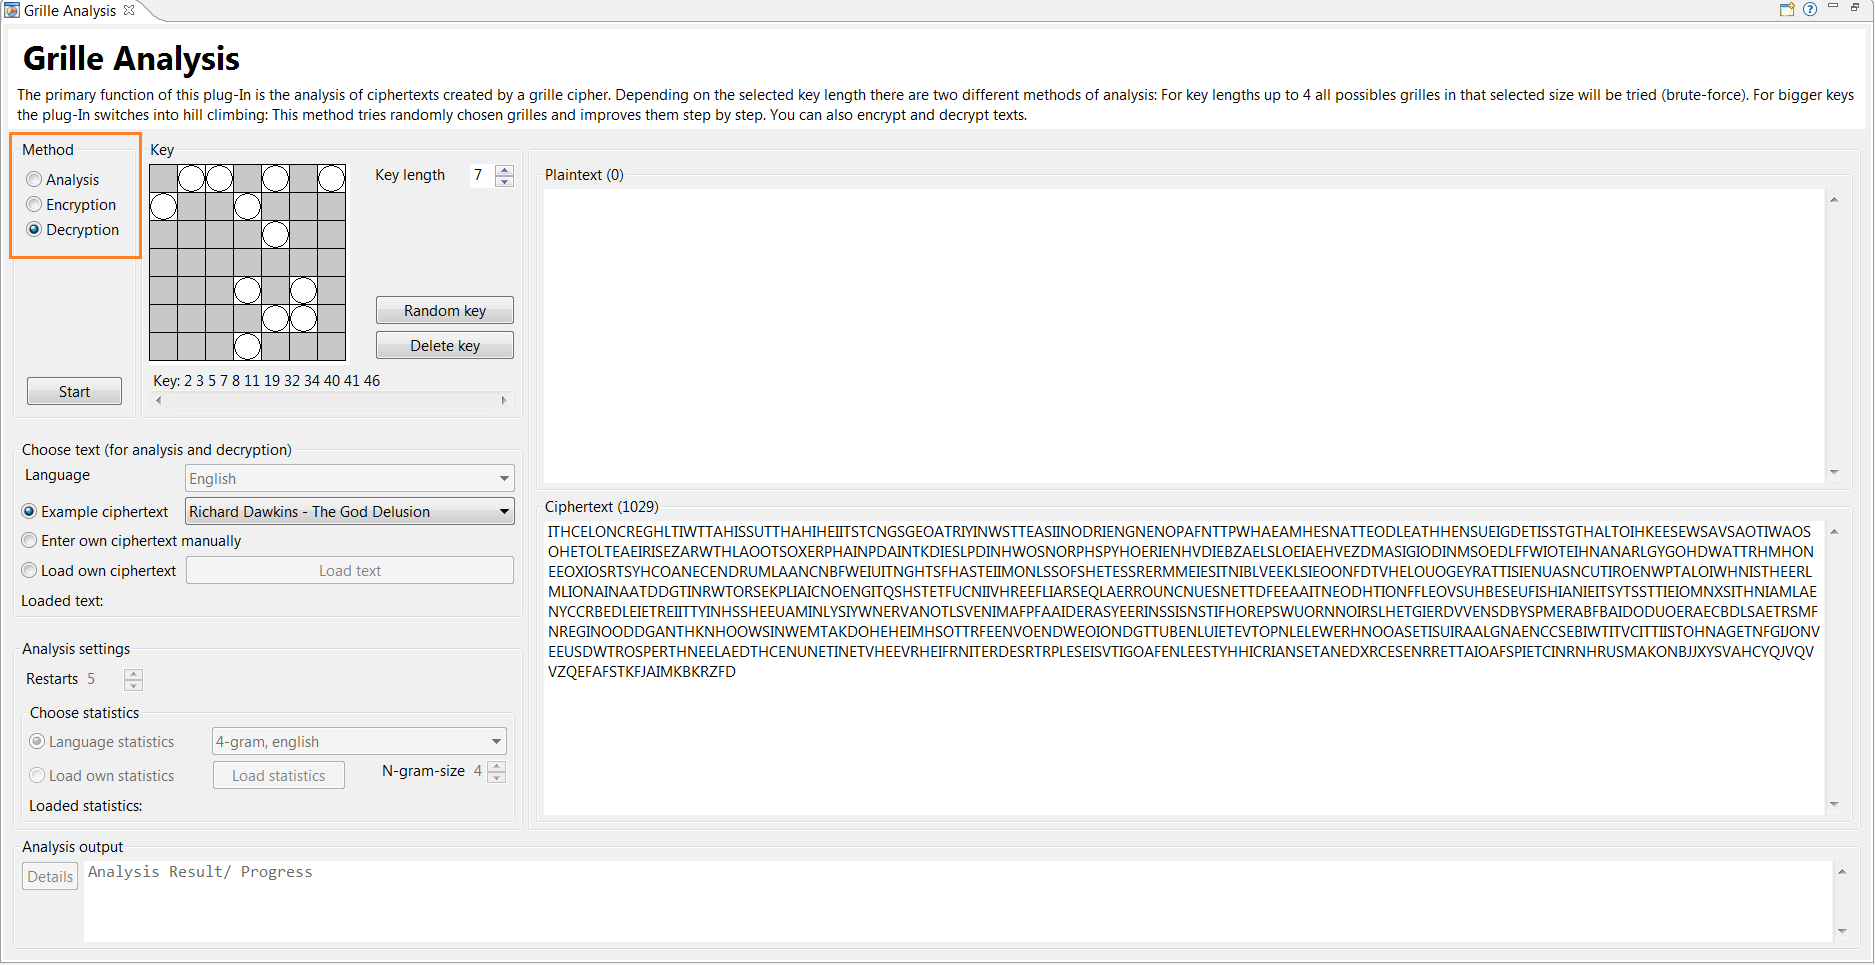
\includegraphics[scale=0.45]{enFleissnerDecrypt.png}

A valid key along with a non-empty ciphertext field and a non-empty plaintext field are required for both decryption and encryption, respectively. The operation of the text selection is analogous to the two methods already described.
\end{document}